% The entire content of this work (including the source code
% for TeX files and the generated PDF documents) by 
% Hongxiang Chen (nicknamed we.taper, or just Taper) is
% licensed under a 
% Creative Commons Attribution-NonCommercial-ShareAlike 4.0 
% International License (Link to the complete license text:
% http://creativecommons.org/licenses/by-nc-sa/4.0/).
\documentclass{article}


% My own physics package
% The following line load the package xparse with additional option to
% prevent the annoying warnings, which are caused by the package
% "physics" loaded in package "physics-taper".
\usepackage[log-declarations=false]{xparse}
\usepackage{physicist-taper}

\makenomenclature
% Followings are for the special character: differential "d".
\newcommand*\diff{\mathop{}\!\mathrm{d}}
\newcommand*\Diff[1]{\mathop{}\!\mathrm{d^#1}}

% Show the keys for labels, replace options with "final" when done
% with editing.
\usepackage[draft,notref]{showkeys}

% Resolve pdf version warning
\pdfoptionpdfminorversion=6

\title{Group Theory in Physics (Course Note)}
\date{\today}
\author{Taper}

\begin{document}


\maketitle
\abstract{
This is our course note for the course about group theoy, with its
application in physics.
}
\tableofcontents
\paragraph{Information about the class}
\begin{enumerate}
    \item Final project: Combine group theory with you research.
    \item Mid-term and final exam.
    \item No homework, cause it is already graduate level.
    \item Professor Fei Ye. (Phone: 88018229, 228 in Research building 2), 
        T.A. Zhe Zhang. (110 Research building 2).
\end{enumerate}

\section{20160919}
\label{sec:20160919}


He first introduces several common examples of symmetries in our life and
physics. Omitted, with one exception:

He mentions that there is one more symmetry in the Hydrogen 
Hamiltonian: the Laplace-Runge-Lenz symmetry. (So its symmetry 
group is not just $SO(3)$, but two copies of $SO(3)$ that forms a $SO(4)$.
And using the representation of $SO(4)$, the complete spectrum of
Hydrogen Hamiltonian is solved. Hence this $SO(4)$ is the largest
symmetry of Hydrogen Hamiltonian.

    \subsection{Digression about Lenz vector}
    \label{sec:Digression_about_Lenz_vector}
    Since the class is too boring, I checked about the Lenz vector via
    Google and found this Math.SE question \cite{math.se_1_lenz_vector}

    The first answer to that post is:

    \begin{center}\noindent\rule{8cm}{0.4pt}\end{center}

    \begin{quote}
        1) \textbf{Problem}. The \href{http://en.wikipedia.org/wiki/Kepler_problem}{Kepler Problem} has Hamiltonian

        $$ H~:=~ \frac{p^2}{2m}- \frac{k}{q},  $$

        where $m$ is the 2-body reduced mass. The [Laplace–Runge–Lenz vector](http://en.wikipedia.org/wiki/Laplace%E2%80%93Runge%E2%80%93Lenz_vector) is (up to an irrelevant normalization)

        $$ A^j ~:=~a^j  + km\frac{q^j}{q}, \qquad a^j~:=~({\bf L} \times {\bf p})^j~=~{\bf q}\cdot{\bf p}~p^j- p^2~q^j,\qquad {\bf L}~:=~ {\bf q} \times {\bf p}.$$ 

        2) \textbf{Action}. The Hamiltonian Lagrangian is

        $$  L_H~:=~ \dot{\bf q}\cdot{\bf p} - H, $$

        and the action is 

        $$ S[{\bf q},{\bf p}]~=~ \int {\rm d}t~L_H .$$

        The non-zero fundamental canonical Poisson brackets are 

        $$ \{ q^i , p^j\}~=~ \delta^{ij}. $$

        3) \textbf{Inverse Noether's Theorem}. Quite generally in the Hamiltonian formulation, given a constant of motion $Q$, then the infinitesimal variation 

        $$\delta~=~ \varepsilon \{Q,\cdot\}$$ 

        is a global off-shell symmetry of the action $S$ (modulo boundary terms). Here $\varepsilon$ is an infinitesimal global parameter, and $X_Q=\{Q,\cdot\}$ is a Hamiltonian vector field with Hamiltonian generator $Q$. The full Noether current is (minus) $Q$, see e.g. my answer to [this question](http://physics.stackexchange.com/q/8626/2451). \hl{(The words \textbf{on-shell}. and \textbf{off-shell}. refer to whether the equations of motion are satisfied or not.)}

        4) \textbf{Variation}. Let us check that the three Laplace–Runge–Lenz components $A^j$ are Hamiltonian generators of three continuous global off-shell symmetries of the action $S$. In detail, the infinitesimal variations $\delta= \varepsilon_j \{A^j,\cdot\}$ read

        $$ \delta  q^i ~=~  \varepsilon_j  \{A^j,q^i\}   , \qquad 
         \{A^j,q^i\} ~ =~ 2 p^i q^j - q^i p^j - {\bf q}\cdot{\bf p}~\delta^{ij}, $$
        $$ \delta  p^i ~=~  \varepsilon_j  \{A^j,p^i\}   , \qquad  
        \{A^j,p^i\}~ =~ p^i p^j - p^2~\delta^{ij} +km\left(\frac{\delta^{ij}}{q}- \frac{q^i q^j}{q^3}\right), $$
        $$ \delta  t ~=~0,$$

        where $\varepsilon_j$ are three infinitesimal parameters.

        5) Notice for later that

        $$ {\bf q}\cdot\delta {\bf q}~=~\varepsilon_j({\bf q}\cdot{\bf p}~q^j - q^2~p^j),  $$

        $$ {\bf p}\cdot\delta {\bf p}
        ~=~\varepsilon_j km(\frac{p^j}{q}-\frac{{\bf q}\cdot{\bf p}~q^j}{q^3})~=~- \frac{km}{q^3}{\bf q}\cdot\delta {\bf q},  $$

        $$ {\bf q}\cdot\delta {\bf p}~=~\varepsilon_j({\bf q}\cdot{\bf p}~p^j - p^2~q^j )~=~\varepsilon_j a^j,  $$

        $$ {\bf p}\cdot\delta {\bf q}~=~2\varepsilon_j( p^2~q^j - {\bf q}\cdot{\bf p}~p^j)~=~-2\varepsilon_j a^j~.  $$

        6) The Hamiltonian is invariant

        $$ \delta  H ~=~ \frac{1}{m}{\bf p}\cdot\delta {\bf p} + \frac{k}{q^3}{\bf q}\cdot\delta {\bf q}~=~0, $$

        showing that the Laplace–Runge–Lenz vector $A^j$ is classically a constant of motion 

        $$\frac{dA^j}{dt} ~\approx~ \{ A^j, H\}+\frac{\partial A^j}{\partial t} ~=~  0.$$   

        (We will use the $\approx$ sign to stress that an equation is an on-shell equation.) 

        7) The variation of the Hamiltonian Lagrangian $L_H$ is a total time derivative

        $$ \delta L_H~=~ \delta  (\dot{\bf q}\cdot{\bf p})~=~ \dot{\bf q}\cdot\delta {\bf p} - \dot{\bf p}\cdot\delta {\bf q} + \frac{d({\bf p}\cdot\delta {\bf q})}{dt} $$
        $$  =~ \varepsilon_j\left( \dot{\bf q}\cdot{\bf p}~p^j - p^2~\dot{q}^j +  km\left( \frac{\dot{q}^j}{q} -  \frac{{\bf q} \cdot \dot{\bf q}~q^j}{q^3}\right)\right)    $$
        $$- \varepsilon_j\left(2 \dot{\bf p}\cdot{\bf p}~q^j - \dot{\bf p}\cdot{\bf q}~p^j- {\bf p}\cdot{\bf q}~\dot{p}^j  \right) - 2\varepsilon_j\frac{da^j}{dt}$$
        $$ =~\varepsilon_j\frac{df^j}{dt}, \qquad f^j ~:=~ A^j-2a^j, $$

        and hence the action $S$ is invariant off-shell up to boundary terms.

        8) \textbf{Noether current}. The bare \href{http://en.wikipedia.org/wiki/Noether%27s_theorem}{Noether current} $j^k$ is

        $$j^k~:=~ \frac{\partial L_H}{\partial \dot{q}^i}  \{A^k,q^i\}+\frac{\partial L_H}{\partial \dot{p}^i}  \{A^k,p^i\}
        ~=~ p^i\{A^k,q^i\}~=~ -2a^k. $$

        The full Noether current $J^k$ (which takes the total time-derivative into account) becomes (minus) the Laplace–Runge–Lenz vector

        $$ J^k~:=~j^k-f^k~=~ -2a^k-(A^k-2a^k)~=~ -A^k.$$

        $J^k$ is conserved on-shell 

        $$\frac{dJ^k}{dt} ~\approx~  0,$$  

        due to \href{http://en.wikipedia.org/wiki/Noether%27s_theorem}{Noether's first Theorem}. Here $k$ is an index that labels the three symmetries.
    \end{quote}

    \begin{center}\noindent\rule{8cm}{0.4pt}\end{center}

    However, I don't really understand the content inside. I asked professor
    Ye whether we can find some physics about this conserved quantity, and
    he answered with no.

    The next answer is also interesting:
    
    \begin{center}\noindent\rule{8cm}{0.4pt}\end{center}

    \begin{quote}
        While Kepler second law is simply a statement of the conservation of angular momentum (and as such it holds for all systems described by central forces), \hl{the first and the third laws are special and are linked with the unique form of the newtonian potential $-k/r$.} In particular, \hl{Bertrand theorem assures that *only* the newtonian potential and the harmonic potential $kr^2$ give rise to closed orbits (no precession).} It is natural to think that this must be due to some kind of symmetry of the problem. In fact, the particular symmetry of the newtonian potential is described exactly by the conservation of the RL vector (\hl{it can be shown that the RL vector is conserved iff the potential is central and newtonian}). This, in turn, is due to a more general symmetry: \hl{if conservation of angular momentum is linked to the group of special orthogonal transformations in 3-dimensional space $SO(3)$, conservation of the RL vector must be linked to a 6-dimensional group of symmetries}, since in this case there are apparently six conserved quantities (3 components of $L$ and 3 components of $\mathcal A$). In the case of bound orbits, this group is $SO(4)$, the group of rotations in 4-dimensional space.  

        Just to fix the notation, the RL vector is:

        \begin{equation} \mathcal{A}=\textbf{p}\times\textbf{L}-\frac{km}{r}\textbf{x} \end{equation}

        Calculate its total derivative:

        \begin{equation}\frac{d\mathcal{A}}{dt}=-\nabla U\times(\textbf{x}\times\textbf{p})+\textbf{p}\times\frac{d\textbf{L}}{dt}-\frac{k\textbf{p}}{r}+\frac{km(\textbf{p}\cdot \textbf{x})}{r^3}\textbf{x} \end{equation}

        Make use of Levi-Civita symbol to develop the cross terms:

        \begin{equation}\epsilon_{sjk}\epsilon_{sil}=\delta_{ji}\delta_{kl}-\delta_{jl}\delta_{ki}   \end{equation}

        Finally:

        \begin{equation}
        \frac{d\mathcal{A}}{dt}=\left(\textbf{x}\cdot\nabla U-\frac{k}{r}\right)\textbf{p}+\left[(\textbf{p}\cdot\textbf{x})\frac{k}{r^3}-2\textbf{p}\cdot\nabla U\right]\textbf{x}+(\textbf{p}\cdot\textbf{x})\nabla U
        \end{equation}

        Now, if the potential $U=U(r)$ is central:

        \begin{equation}
        (\nabla U)_j=\frac{\partial U}{\partial x_j}=\frac{dU}{dr}\frac{\partial r}{\partial x_j}=\frac{dU}{dr}\frac{x_j}{r}
        \end{equation}

        so 

        \begin{equation} \nabla U=\frac{dU}{dr}\frac{\textbf{x}}{r}\end{equation}

        Substituting back:

        \begin{equation}
            \hlMath{\frac{d\mathcal A}{dt}=\frac{1}{r}\left(\frac{dU}{dr}-\frac{k}{r^2}\right)[r^2\textbf{p}-(\textbf{x}\cdot\textbf{p})\textbf{x}]}
        \end{equation}

        Now, you see that if $U$ has \textit{exactly} the newtonian form then the first parenthesis is zero and so the RL vector is conserved. 

        Maybe there's some slicker way to see it (Poisson brackets?), but this works anyway.
    \end{quote}
    \begin{center}\noindent\rule{8cm}{0.4pt}\end{center}
    
    % TODO Study in detail about this example.

    \subsection{Coming back to the course}

After mentioning the Poinc\'{a}re group, he produces to review some
concepts about linear algebra:
\begin{enumerate}
    \item The axioms of linear space, using quantum mechanics
        as basic example (Omitted).
    \item Some common concepts of linear space: linear-independence,
        subspace, direct sum, linear operators, its matrix representation. (Omitted)
    \item Introducing the complete antisymmetric tensor 
        $\epsilon^{a_1,\cdots,a_n}$. Some properties:
        \begin{align}
            \frac{1}{(m-n)!} \sum_{a_{n+1},\cdots, a_m}
            & \epsilon_{a_1,\cdots,a_n,a_{n+1},a_m}
            \epsilon_{b_1,\cdots,b_n,a_{n+1},a_m}\nonumber
            \\
            &= \sum_{p_1,\cdots,p_n} 
            \epsilon_{p_1,\cdots,p_n} 
                \delta_{a_1,b_{p_1}}\cdots \delta_{a_n,b_{p_n}}
                \\
            \epsilon_{ab}\epsilon_{rs} &=
                \delta_{ar}\delta_{bs}-\delta_{as}\delta_{br}
                \\
            \sum_d\epsilon_{abd}\epsilon_{rsd} &=
                \delta_{ar}\delta_{bs} + \delta_{as}\delta_{br}
        \end{align}
    \item Some special matrices.
    \item Fact: If $R\Gamma = \Gamma R$, and 
        $\Gamma$ is diagonal. (let $\mu\neq\nu$) Then if 
        $\Gamma_{\mu\mu} \neq \Gamma_{\nu\nu}$ , we have:
        $ R_{\mu\nu}=R_{\nu\mu} = 0 $.
        On the other hand, if $R_{\mu\nu}\neq 0$, then
        $\Gamma_{\mu\mu}=\Gamma_{\nu\nu}$.
        This is obviously from:
        \begin{align*}
            \sum_j R^{i}_{j}\Gamma^{j}_{k}=\sum_j\Gamma^{i}_{j} R^{j}_k
            \Longrightarrow
            R^i_k\Gamma^k_k = \Gamma^i_i R^i_k
        \end{align*}
        where the first is automatically summed, and the second is not.

    \item A linear functional is closed w.r.t. a vector space. (Omitted)
    \item ... then this linear functional can be expressed as a
        matrix w.r.t to a basis of this vector space. (Omitted)
    \item Invariant subspace. (Omitted)
    \item Transformation of basis. (Omitted)
    \item Direct sum of operators:

        Let vector spaces $L=L_1\oplus L_2$, with $L=\braket{e_i}$,
        $L_1=\braket{e'_1,\cdots e'_n}$,$L_2=\braket{e'_{n+1},\cdots,e'_m}$,
        $e'_\nu=\sum_\mu e_\mu  S_{\mu\nu}$. 
        Assume that $L_1,L_2$ are invariant w.r.t $A$, an linear operator. If:
        \begin{align}
            A e'_\mu = \sum_{\nu=1}^{m} e'_\nu R'_{\nu\mu}
        \end{align}
        we have obviously:
        \begin{align}
            A e'_\mu = \sum_{\nu=1}^{n} e'_\nu R'_{\nu\mu} \text{for }
                \mu\in \{1\cdots n\}
                \\
            A e'_\mu = \sum_{\nu=n}^{m} e'_\nu R'_{\nu\mu} \text{for }
                \mu\in \{n\cdots m\}
        \end{align}
        i.e., $A$'s matrix representation has two diagonal blocks.
        Using this fact, $A$ after a linear transformation (by $S$),
        could be written as $R_1\oplus R_2$, where the meaning of $R_1/R_2$
        is obvious.
    \item Eigenvalues and the characteristic equation. (Omitted)
        Some properties:
        \begin{enumerate}
            \item Trace = $\sum_i \lambda_i$
            \item Determinant = $\prod_i \lambda_i$
            \item Geometric multiplicity $\leq$ Algebraic multiplicity, or
                $$\mathrm{dim}V_{\lambda_1} \leq n_1$$.
        \end{enumerate}
    \item Inner product and orthonormal basis. (Omitted) Here we define
        matrix $\Omega$ to be, when a basis $\{e_i\}$is given:
        \begin{defi}[]
        \nomenclature{}{\nomrefpage.}
            \begin{align}
                \Omega_{ij} \equiv \braket{e_i,e_j}
            \end{align}
        \end{defi}
    \item Adjoint operator:

        Let $A$ be a linear operator represented by matrix $A^i_j$. Let
        its adjoint $A^\dagger$ be represented by $R^i_J$. Then using
        $\braket{A^\dagger e_j, e_i} = \braket{e_j,A e_i}$, we will
        get $(R^{k}_j)^* \Omega_{ki}= \Omega_{jk}A^k_i$, i.e.
        $(R^T)^* \Omega = \Omega A$, so:
        \begin{align}
            R = \Omega^{-1} A^\dagger \Omega
        \end{align}
        where we have used the fact that $\Omega^\dagger=\Omega$.

        Note that $(R^{k}_j)^* \Omega_{ki}$ is not $\Omega^T R^*$.
        (Be careful and you will find out why.)

        This is very different from my previous naive concept
        when $\Omega$ is not identity matrix, i.e. when the basis
        is not orthonormal.
\end{enumerate}



\section{20160926}
\label{sec:20160926}
He first introduces some important matrices:

\subsection{Some Important Matrices}
\label{sec:Some-Important-Matrices}

\paragraph{Unitary matrix} Eigenvalues of Unitary matrices has modulus $1$,
i.e. $|\lambda|=1$. This can be proved directly. Also, Unitary matrices are unitarily diagonalizable. This is a result of the following Spectral Theorem:
\begin{thm}[Spectral Theorem]
    One matrix $A$ is normal (i.e. $A^\dagger A= AA^\dagger$), if and only if it is unitarily diagonalizable.
\end{thm}
\begin{proof}
    If $A$ is normal, then by Schur decomposition, we can write
    $A=UTU^\dagger$, here $U$ is unitary and $T$ is upper-triangular. 
    Using the condition of being normal, one can show directly that $T$ 
    is in fact also normal. Now we show that any triangular matrix that 
    is normal must be diagonal. Observe that we have 
    $\braket{e_i,T^\dagger T e_i}=\braket{e_i,TT^\dagger e_i}$, 
    i.e. $\braket{T^\dagger e_i, T^\dagger e_i}=\braket{T e_i, T e_i}$. 
    This is saying that the norm of the first column of $A^\dagger$ 
    is equal to the norm of the first column of $A$. Obviously 
    $A$ has to be diagonal.

    The converse is obvious.
\end{proof}

Also, unitary matrix's eigenvector corresponding to different eigenvalues 
are orthogonal. This is a direct result of fact mentioned above.

\paragraph{Hermitian matrices} They have real eigenvalues and orthogonal
eigenvectors (proof omitted). Also, if $\text{det}(R^\dagger R)\neq 0$,
then $R^\dagger R >0$, i.e. it is positive-definite. 

\textbf{This is wong:} An example is that
the matrix $\Omega$ introduced in the previous lecture has
$\text{det}(\Omega^\dagger \Omega)=\text{det}(\Omega)$, hence
$\text{det}(\Omega)=1$ (it cannot be $0$), hence it is positive definite.

\textbf{Actually} 
$\text{det}(\Omega^\dagger \Omega)\neq\text{det}(\Omega)$, because
\begin{align}
    \sum_\rho \ket{e_\rho}\bra{e_\rho} \neq 1 \text{(unless the basis is
        orthonormal)}
    % TODO think about this in depth
\end{align}
Therefore we need anthoer argument for $\Omega$ being positive-definite.
It is provided in page 11 of \cite{book}.

\paragraph{Orthogonal matrix} For an orthogonal matrix over $\mathbb{C}$,
it is quite troublesome. For example, if $Ra=\lambda a$ and
$\lambda \neq \pm 1$, then we have $a^T a=0$, which is quite bad because
this force $a$ to have complex components.

\paragraph{Orthogonal matrix over $\mathbb{R}$} In this case, we have
similar result. But it is easy to show that for an orthogonal matrix
$R$ having only real elements, then its eigenvalues $\lambda= \pm 1$.

Then he proceeds to direct product.
\paragraph{Direct product} and also the Kronecker Product of two
matrices. Properties (let $T=R\otimes S$):
\begin{enumerate}
    \item $\mathrm{dim}T = \mathrm{dim}R \times \mathrm{dim}S$
    \item $\mathrm{tr}(T)=\mathrm{tr}(R)\mathrm{tr}(S)$
    \item $\otimes$ commutes with the operation of inverse, transpose,
        and transpose conjugation.
    \item \begin{align}
            \frac{d}{d\alpha} (R(\alpha)\otimes S(\alpha)) =
            R'(\alpha)\otimes S(\alpha) + R(\alpha)\otimes S'(\alpha)
    \end{align}
    \item when the dimentions are the same:
        \begin{enumerate}
            \item 
            $(R_1\otimes S_1)(R_2\otimes S_2) = (R_1R_2)\otimes (S_1S_2)$
        \end{enumerate}
\end{enumerate}

\subsection{Symmetry and Group}
\label{sec:Symmetry-and-Group}

Finally we arrived in the group theory.
\paragraph{Symmetry examples} Dipole transition. 
$\braket{\phi_f|\hat{P}|\phi_i}$, must happen when the parity of $\phi_i$
and $\phi_f$ is of opposite parity. (pp.18 of \cite{book})

\paragraph{Group}
\begin{defi}[Group]
\nomenclature{Group}{\nomrefpage.}
    Omitted.
\end{defi}
Some basic properties (Omitted).
\begin{defi}[Abel Group]
\nomenclature{Abel Group}{\nomrefpage.}
    Omitted.
\end{defi}
\begin{defi}[Cardinality of group $\# A$]
\nomenclature{Cardinality of group $#$}{\nomrefpage.}
    Omitted.
\end{defi}

\paragraph{Multiplication table}

Facts: group of order $1,2,$ and $3$ are unique up to an isomorphism.

\begin{defi}[Cyclic group, generators]
\nomenclature{Cyclic group, generators}{\nomrefpage.}
    Omitted.
\end{defi}

\begin{CJK}{UTF8}{gbsn}
固有转动是指的那些 $det(M)>0$ 的转动. 用$C_n$来表示他们.

Also, 周期 of $R$ is just $\braket{R}$.
\end{CJK}

Let $\sigma$\nomenclature{$\sigma$}{\nomrefpage.} for spatial reflection.
\begin{defi}[$C_N,\bar{C}_N$]
\nomenclature{$C_N,\bar{C}_N$}{\nomrefpage.}
    $\bar{C}_N=C_N*\sigma$
\end{defi}


\section{20161010}
\label{sec:20161010}

\subsection{Common Concepts in Group}
\label{sec:Common-Concepts-in-Group}

Introducing to various groups:$S_4, V_4$, $D_3$, all omited.
(\textbf{pp.22-23 of \cite{book}})

$D_n$ group. See pp. 25-26 of the book \cite{book}.
Note that here the $n$ refers to the $n$-polygon, not that the group is
of order $n$. For the mathematicians, they might be comfortable with
$D_n$ means the dihedral group of order $n$, but is actually the group of
symmetries of $n/2$-polygon.

\begin{defi}[Subgroup]
\nomenclature{Subgroup}{\nomrefpage.}
    Omitted.
\end{defi}
\begin{fact}
    One only has to check the closeness for determining a subgroup, if it
    is of finite order.

    However, for group of infinite order, one has to check the existance
    of unit and inverse elements.
\end{fact}
Examples of subgroup (\textbf{pp.26 of \cite{book}})

Noteworth:$C_6$ has three copies of $D_2$, this can be intuitively 
guessed by the fact that a hexago has three rectanle in it.

\begin{defi}[Coset]
\nomenclature{Coset}{\nomrefpage.}
    Omitted.
\end{defi}
Properties of coset (omitted).

\begin{defi}[Index of subgroup]
\nomenclature{Index of subgroup}{\nomrefpage.}
    Omitted.
\end{defi}

\begin{prop}
    Two elements $R$ and $T$ belongs to the same coset $kH$, if and only
    if $R^{-1}T\in H$.
\end{prop}
\begin{proof}
    Omitted.
\end{proof}
\begin{defi}[Normal/Invariant subgroup]
\nomenclature{Normal/Invariant subgroup}{\nomrefpage.}
    A subgroup is normal or nnvariant subgrouproup(also invariant), if
    and only if for any $x\in G$, we have $xH = Hx$.
\end{defi}
\begin{fact}
    If $H$ has index 2, then it must be normal/invariant. This is
    obvious.
\end{fact}
\begin{defi}[Quotient]
\nomenclature{Quotient}{\nomrefpage.}
    Omitted.
\end{defi}
Note that quotient group (a.k.a. factor group) is only defined for a normal subgroup.

\begin{ex}
    $D_3$ (Using the multiplication table). Omitted because it is too
    complex to be typed down here.
\end{ex}

\subsection{Conjugacy classes}
\label{sec:Conjugacy-classes}

\begin{defi}[Conjugate]
\nomenclature{Conjugate}{\nomrefpage.}
    If exists $S\in G$, s.t. $R' = S^{-1}RS$, then we say $R'$ is
    conjugate to $R$.
\end{defi}
see (\textbf{pp.28-30 of \cite{book}})
This is clearly an equivalence relationship. By this we can define
conjugate class, denoted by $C=\{R_1,\cdots\}$, then we have the
characterization $C = \{ s^{-1} R_i s|\forall s\in G\}$, for any
$R_i$. We then have the following facts (all are obvious):
\begin{fact}
The unit class formed just by the unit element.
\end{fact}
\begin{fact}
    The inverse class formed by just all the inverse element.  $C^{-1}
    = \{ R_i^{-1}\}$. If $C\cap C^{-1}\neq\varnothing$, then
    $C=C^{-1}$, $C$ is called self-inverse\nomenclature{self-inverse
    class}{\nomrefpage}.
\end{fact}
\begin{fact}
    The order of elements in a class is just the same.
\end{fact}
\begin{fact}
    For $\forall T,S\in G$, $TS$ and $ST$ are conjugate to each other.
    This means that all elements symmetric on the multiplication table is
    conjugate to each other.
\end{fact}
\begin{fact}
    For two elements $R$, $R'$ conjugate to each other, both can be
    expressed by the products of two elements in two different way. (Isn't
    this too obvious to mention.)
\end{fact}
\begin{fact}
    \label{fact:20161010-srs}
    Let $G$ be a rotation group. Suppose it has an axis of the
    order of $n$, with its operation denoted as $R$,, we can get a
    new axis by the following steps. (Supose we have another
    rotation $S$),
    \begin{enumerate}
        \item  $S^{-1}$, rotate $m$ back to $n$.
        \item  $R$, rotate about n around $2\pi/n$,
        \item  $S$ rotate $n$ to $m$
    \end{enumerate}

    Result: $S^{-1}RS$ rotate around a new axis $m$ about
    $2\pi/n$. So $R'=S^{-1}RS$ and $R$ is calle the equivalent
    axis. 
    
    Also, if $m=-n$, then they are called polar axis to each
    other.
\end{fact}
\begin{fact}
    $C_n$, which is an abel group, every element form a conjugate
    class by itself. Specifically, $e$ and $R^{n/2}$ are self inverse,
    if $n$ is even.
\end{fact}

\begin{prop}
    \label{prop:20161010.conjugate_subgroup}
    For an normal subgroup, every conjugate element is also
    inside the same normal subgroup. This indicates that an normal
    subgroup can be decomposed into a series of sum of conjugate classes.
\end{prop}
\begin{proof}
    If $R\in H$, then we show that $S^{-1}RS\in H$, this is obviously
    since it belongs to $S^{-1}HS$.
\end{proof}

\begin{ex}
    For $D_3: E,D,F,A,B,C$, their orders are respetively
    $1,3,3,2,2,2$. We have the following conjugate classes:
    \begin{enumerate}
        \item $\{ E\}$. Is self inverse.
        \item $\{ D,F\}$. $D$ is conjugate to $F$. We can see
            this physically by looking at rotation from the front
            or the below. This class is also self-inverse.
        \item $\{A,B,C\}$, is clearly a self-inverse conjugate
            class.
    \end{enumerate}
\end{ex}
\begin{ex}[$D_6$]
    Ramiliarize one with the formulae for $D_n$. Hint: use the order of
    elements to find classes of conjugate. Then use the proposition
    \ref{prop:20161010.conjugate_subgroup} to find the subgroups.
    % TODO maybe I can try this when I am free.
\end{ex}







\section{Skipped Two lectures}

Due to GRE physics preparation. Concepts that may have been covered:

\begin{itemize}
    \item Conjugacy classes
    \item Representation of Groups.
        \begin{itemize}
            \item Character of representation. (Notes for this part is
                delayed to be contained in the next lecture's note).
            \item Equivalence between representation.
        \end{itemize}
    \item Transformation of Fields
    \item Group Algebra and Regular Representation.
\end{itemize}

\subsection{Conjugacy classes (continued)}
\label{sec:Conjugacy classes (continued)}

One important group is the symmetric group. It is important because
that every finite group of order $n$ can be embedded inside the
symmetric group $S_n$ (Cayley's theorem) \footnote{
    However, it is hard sometimes to find the smallest possible
    symmetric group to embed into. For example, $S_3$ has 6 elements
    and can thus be embedded into $S_6$. But obviously it can be
    embedded better just into itself $S_3$.
}.

The conjugacy classes in symemtric is pretty easy to find. What we
need to know is the following observation (from \cite{Ludeling})

\begin{key}
    Consider two permutation $\pi$ and $\sigma$:
    \begin{align}
        \pi =\left( \begin{array}{ccc}
             1 & \cdots & n \\
            \pi(1) & \cdots & \pi(n) \\
            \end{array} \right) ,\quad\quad
        \sigma = \left( \begin{array}{ccc}
             1 & \cdots & n \\
            \sigma(1) & \cdots & \sigma(n) \\
            \end{array} \right)
    \end{align}
    Then we have by direct calculation:
    \begin{align}
        \sigma\pi\sigma^{-1} = \left( \begin{array}{ccc}
                \sigma(1)      & \cdots & \sigma(n) \\
                \sigma(\pi(1)) & \cdots & \sigma(\pi(n)) \\
            \end{array} \right)
    \end{align}
    Therefore, the cycle structure of $\pi$ is unchanged under any
    "conjugacy transformation".
\end{key}
What do I mean by cycle structure? Let's see an example. Suppose we
have a cycle $(123)$:
\begin{center} \begin{tikzcd}[column sep=small]
    & 1 \arrow[dr] & \\
    2\arrow[ru] & & 3\arrow{ll} 
\end{tikzcd} \end{center}
Then the conjugated map $\sigma (123) \sigma^{-1}$ will have:
\begin{center} \begin{tikzcd}[column sep=small]
    & \sigma(1) \arrow[dr] & \\
    \sigma(2)\arrow[ru] & & \sigma(3)\arrow{ll} 
\end{tikzcd} \end{center}
So it has a cycle of $(\sigma(1)\sigma(2)\sigma(3))$.
We see that in general, the cycle type is unchanged under conjugacy
transformation.
\footnote{ For a permutation, its cycle type is determined by
    decomposing it into independent cycles. For independent cycles,
    the cycle type is unique. For example, $(135)(24)$ has a cycle
    type of $(3,2)$, or $(2,3)$ since the order is irrelevant. But if
    we decompose it into non-independent cycles, we cannot determine
    its cycle type. For example, $(135)=(15)(13)$, which is ambiguous
    if we were to tell the cycle type.
}

On the other hand, all elements of the same cycle type belong to the
same conjugacy class. For example, consider two permutations:
$(i_1 i_2 i_3)(i_4 i_5)$ and $\left(\pi_{i_1}
\pi_{i_2}\pi_{i_3}\right)\left(\pi_{i_4}\pi_{i_5}\right)$, where $\pi$
permutes the five numbers $i_1 \cdots i_5$.
Consider the map:
\begin{equation}
    \sigma \equiv \left( \begin{array}{ccc}
            i_1      & \cdots & i_5 \\
            \pi_{i_1} & \cdots & \pi_{i_5} \\
        \end{array} \right)
\end{equation}
Then \begin{align*}
    &\sigma (i_1 i_2 i_3)(i_4 i_5) \sigma^{-1} =  \\
    &\left( \begin{array}{ccc}
            i_1      & \cdots & i_5 \\
            \pi_{i_1} & \cdots & \pi_{i_5} \\
        \end{array} \right)
        (i_1 i_2 i_3)(i_4 i_5)
        \left( \begin{array}{ccc}
            \pi_{i_1} & \cdots & \pi_{i_5} \\
            i_1      & \cdots & i_5 \\
        \end{array} \right) \\
    & = (\pi_{i_1} \pi_{i_2}\pi_{i_3})(\pi_{i_4}\pi_{i_5})
\end{align*}
The proof for the general case is similar. So we have the theorem
below:
\begin{thm}[Cycle type determines conjugacy class]
    Two permutations are conjugate in the symmetric group if and only if they have the same cycle type.
\end{thm}
\begin{remark}
    \label{rmk:20161010-conjugacy_class_in_Sn}
    Since a cycle type is just a set of unordered integer partition of
    number $n$. The above theorem means that the set of conjugacy
    classes in the symmetric group on a finite set is in bijection
    with the set of unordered integer partitions of the size of the
    set. 
\end{remark}

\subsection{Group Representation}
\label{sec:Group-Representation}

\begin{defi}[Representation]
\nomenclature{Representation}{\nomrefpage.}
    A representation of a group $G$ is a continuous homomorphism $D$
    from $G$ to the group of automorphisms of a vector space $V$:
    \begin{equation}
        D: G\mapsto \mathrm{Aut}V
    \end{equation}
    $V$ is called the \textit{represetation space}, and the
    \textit{dimension of the representation} is the dimension of $V$.
\end{defi}

Related concepts. (The following is copied from \cite{Ludeling}.)

\begin{itemize}
    \item There is always the representation $D(g) = 1$ for all $g$.
        If $\mathrm{dim} V = 1$, this is called the \textit{trivial
        representation} \nomenclature{trivial
        representation}{\nomrefpage}.
    \item The matrix groups, i.e. $\mathrm{GL}(n, K)$ and subgroups,
        naturally have the representation "by themselves", i.e.
        by$n\times n$ matrices acting on $K_n$ and satisfying the
        defining constraints (e.g. nonzero determinant). This is
        loosely called the \textit{fundamental or defining
        representation}.
    \item Two representations $D$ and $D'$ are called
        \textit{equivalent}\nomenclature{equivalent of
        representation}{\nomrefpage} if they are related by a
        similarity transformation, i.e. if there is an operator S such
        that
        \begin{equation}
            SD(g)S^{-1} = D'(g)
        \end{equation}
        for all $g$. Note that $S$ does not depend on $g$! Two equivalent
        representation can be thought of as the same representation in
        different bases. We will normally regard equivalent
        representations as being equal.

        Note also here $S$ represents a transformation of vector. If we
        know the transformation of basis $X$, then
        \begin{equation}
            X^{-1} D(g)X = D'(g)
        \end{equation}
    \item A representation is called
        \textit{faithful}\nomenclature{faithful
        representation}{\nomrefpage} if it is injective, i.e.
        $\mathrm{ker} D = \{e\}$, or in other words, if $D(g_1) \neq
        D(g_2)$ whenever $g_1 \neq g_2$.
    \item If $V$ is equipped with a (positive definite) scalar
        product, D is unitary if it preserves that scalar product, i.e
        if
        \begin{equation}
            \braket{u,v} = \braket{D(g)u,D(g)v}
        \end{equation}
        for all $g\in G$. (Here we assume that $V$ is a complex vector
        space, as that is the most relevant case. Otherwise one could
        define orthogonal representations etc.)
\end{itemize}

\subsubsection{Regular Representation}
\label{sec:Regular-Representation}

Now we construce a simple representation for all groups. It utilizes a
vector space constructed from group itself called Group Algebra.

\begin{defi}[Group algebra/Monoid algebra]
\nomenclature{$A[G]$ group algebra/monoid algebra}{\nomrefpage.}

    Let $A$ be a commutative ring, $G$ be a monoid, written
    multiplicatively. Then the monoid ring $A[G]$ consists of those
    finite formal linear combinations $v$ of the form:
    \begin{equation}
        v = \sum_{g\in G} v_g g
    \end{equation}
    where $v_g \in A$. The $v_g$ are seen as coefficients and $g$ are
    seen as the basis vectors that can be multiplied. Soe the addition
    is defined as:
    \begin{equation}
        v+w = \sum_{g\in G} (v_g + w_g) g
    \end{equation}
    And the multiplication is
    \begin{equation}
        v w = \sum_{g,g'\in G} (v_g w_{g'}) gg'
    \end{equation}
    If $G$ is a group then the
    corresponding $A[G]$ is called a \textit{group algebra}.
\end{defi}
A rigorious definition would use the concept of function to define the
"formal linear combination". Please refer to page 105 (section II.3) of
\cite{lang-algebra}. 
\begin{remark}
    Note that both $A$ and $G$ can be naturally embeded into $A[G]$.
    This will helps us to define a representation of group $G$ later.
\end{remark}

\begin{ex}
    (From page 106 of \cite{lang-algebra}.)
    Polynomial rings are special cases. In $n$ variables, consider a
    multiplicative free abelian group of rank $n$. Let $X_l,\cdots
    X_n$ be generators. Let $G$ be the multiplicative subset
    consisting of elements $X_1^{v_1},\cdots,X_n^{v_n}$, where
    $v_i\leq 0$ for all $i$. Then $G$ is a monoid, and it is eas to
    verify that $A[G]$ is just $A[X_1,\cdots, X_n]$.
\end{ex}

Here we take $A$ to be $\mathbb{C}$, then we have clearly
$\mathbb{C}[G]$ a vector space equipped with a bilinear map (the
product), i.e. an algebra over a field. Its dimension is clear equal
to the order of $G$. We can also give it an inner product by:
\begin{equation}
    \braket{v,w} =\sum_{g\in G} v_g^* w_g
\end{equation}
Now we can define the regular representation:

\begin{defi}[Regular Representation]
\nomenclature{Regular Representation}{\nomrefpage.}
    A regular representation of a group $G$ is the following
    endomorphism of $\mathbb{C}[G]$:
    \begin{equation}
        D_\text{reg}: v \mapsto g\cdot v
    \end{equation}
    where $v\in \mathbb{C}[G]$, $g\in G \hookrightarrow \mathbb{C}[G]$.
\end{defi}

\begin{remark}
    This representation can be just seen as a permutation of basis
    vectors, because:
    \begin{equation}
        g\cdot v = \sum_{h\in G} v_h (gh) = \sum_{h'\in G}
        v_{g^{-1}h'}\, h'
    \end{equation}
    Therefore, it is unitary.
\end{remark}



\section{20161031}
\label{sec:20161031}


\subsection{Unitarity of Representation}
\label{sec:Unitarity-of-Representation}

\begin{thm}[Unitary Representation]
    For finite groups and for compact Lie groups, all representations
    are equivalent to a unitary representation.
\end{thm}
\begin{remark}
    Before the formal proof, I remarked that since any finite group
    can be embedded inside the symmetric group (Cayley's theorem), and
    the symmetric has clearly a unitary representation (perhaps the
    easiest representation one could ever construct besides the
    trivial representation), one could naturally guess whether it is
    possible that any representation could be turned into a unitary
    one.

    As for the compact Lie group case, it is just mentioned in
    \cite{Ludeling} and will not be proved here. It is mentioned in
    page 25 of \cite{Ludeling} that:
    \begin{quote}
        For compact Lie groups, however, there exists a (unique)
        translationally invariant measure, so we can replace
        $\sum_g\to \int \dd g$ and the integral is convergent because
        of compactness. Then the proof directly carries over.
    \end{quote}
\end{remark}
\begin{proof}
    For $D(g)$, we need to find a $X$ such that $\bar{D}(g)\equiv
    X^{-1}D(g)X$ is unitary.

    Since
    \begin{align*}
        1 = \bar{D}^\dagger \bar{D}
    \end{align*}
    One will find 
    $$ (XX^\dagger)^{-1} = D^\dagger (XX^\dagger)^{-1} D$$
    Then let
    \begin{equation}
        H\equiv \sum_{s\in G} D^\dagger(s) D(s)
    \end{equation}
    One can verify that
    \begin{equation}
        D^\dagger (g) H D(g) = H
    \end{equation}

    Now we construct $X$ from $H$. We have
    \begin{equation}
        H = (XX^\dagger)^{-1}
    \end{equation}

    Notice we have $H$ is Hermitian by above equation. Also, $H$ is
    positive definite (easily seen from the definition of $H$ and 
    $a^\dagger H a \geq 0$. Also $H$ is of full rank.).

    Then we have $UHU^{-1} = \mathrm{diag}\{\gamma_1,\gamma_2,\cdots\}$
    and $\gamma_i > 0$. The rest for constructing $X$ should be
    obvious.
\end{proof}
\begin{remark}[Examples of Non-unitary representation]
    It is remard in \cite{Ludeling} that for infinite and non-compact
    groups, the representation are not unitary in general. He gives
    two examples:
    \begin{itemize}
        \item The group $\mathbb{Z}^*$ acting on $\mathbb{C}$ by
            mulplication is certain not equivalent to any unitary
            representation.
        \item Arugment for a representation of non-compact Lie group
            cannot be made unitary by a similarity transformation:
            \begin{quote}
                The group of unitary operators on a finite dimensional
                vector space is isomorphic to $U(n)$ (for complex
                vector spaces, $O(n)$ otherwise), and is hence
                compact. But there cannot be a bijective continuous
                map between a compact and a non-compact space, so
                faithful finite-dimensional representations of
                non-compact groups will be non-unitary. 
            \end{quote}
            But then he mentions something about a perculiar case, the
            Lorentz group, which I do not understand. 
    \end{itemize}
\end{remark}
Anyway, he summarised in the following:
\begin{quote}
   To summarise, for finite groups and for compact Lie groups, all
   representations are equivalent to a unitary one (and we will
   usually take them to be unitary from now on).  For infinite groups
   and non-compact Lie groups, on the other hand, finite-dimensional
   faithful representations are never unitary. Finally, some
   non-compact groups may have representations which are unitary with
   respect to a non-definite scalar product, such as the Lorentz group 
\end{quote}

From class, Ye Fei proved that:
\begin{thm}
    For any two equivalent representation, there is always a unitary
    matrix to relate the two, i.e. exits $Y$ unitary, s.t.
    $$ \bar{D}(g) = Y^{-1} D(g) Y$$
\end{thm}
\begin{proof}
    Suppose we have two unitary representation $D(g)$ and
    $\bar{D}(g)$, related by
    $$ \bar{D}(g) = X^{-1} D(g) X$$
    where $X$ is not necessarily unitary.

    Let $H\equiv X^\dagger X$, it is easy to prove that $H$ is
    Hermitian and positive definite. Direct calculation shows that
    $$ \bar{D}^{-1}(g) H \bar{D}(g) = H$$
    That is $\bar{D}(g)$ and $H$ commute.
    Then we construct $Y$ from $H$. Let $V$ be such that
    \begin{equation}
        V^{-1} H V = \Gamma
    \end{equation}
    where $\Gamma$ is a diagonal matrix of $H$'s eigenvalues.
    Obviously $V$ has to be unitary. Define $\bar{Y}$ to be
    \begin{equation}
        \bar{Y}\equiv V \sqrt{\Gamma} V^{-1}
    \end{equation}
    By direct calculation, we have
    $$ (X\bar{Y})^\dagger (X\bar{Y}) = \id$$
    One can show that
    $$ \bar{Y}^{-1} \bar{D} \bar{Y} = \bar{D}$$
    with laborious calculation. Then one can easily verify that
    $Y\equiv \bar{Y}X$ is the required unitary transformation.
\end{proof}

\subsection{Reduciblility of Representations}
\label{sec:Reduciblility-of-Representations}

\begin{defi}[Reducible/Irreducible Representation]
    \nomenclature{Reducibility of Representation}{\nomrefpage.}
    A representation $D$ is called \textit{reducible} if $V$ contains an
    invariant subspace. Otherwise $D$ is called irreducible.

    A representation is called \textit{fully reducible} if $V$ can be
    written as the direct sum of irreducible invariant subspaces, i.e.
    $V=V_1\oplus \cdots \oplus V_p$, all the $V_i$ are invariant and the
    restriction of $D$ to each $V_i$ is irreducible.
\end{defi}

\begin{ex}
    The regular representation mentioned before is reducible. For
    example, the vector
    \begin{equation}
        V = \sum_{g\in G} g
    \end{equation}
    spans an invariant subspace of the operator $D_\text{reg}$.
\end{ex}


\begin{ex}$ $

    \begin{itemize}
        \item The representation of finite group is obviously fully
            reducible or irreducible (since a unitary matrix cannot
            have off diagonal blocks).
        \item The representation of translation group is not fully
            reducible. For example, for translation we have:
            $T_a T_b = T_{a+b}$,
            One can confirm that the following representation obeys
            the above relationship:
            $$T_a = \left( \begin{array}{cc}
                 1 & a \\
                 0 & 1 \\
            \end{array} \right)$$
            but this is obviously not fully reducible.
    \end{itemize}
\end{ex}

\begin{defi}[Interwiner]
\nomenclature{Interwiner}{\nomrefpage.}
    Given two representations $D_1$ and $D_2$ acting on $V_1$ and
    $V_2$, an intertwiner between $D_1$ and $D_2$ is a linear operator
    \begin{equation}
        F: V_1 \mapsto V_2
    \end{equation}
    which "commutes" with $G$ in the sense that
    \begin{equation}
        F D_1(g) = D_2(g) F
    \end{equation}
    for all $g\in G$.
\end{defi}

(From pp.30 of \cite{Ludeling})

The existence of an intertwiner has a number of consequences. First,
$D_1$ and $D_2$ are equivalent exactly if there exists an invertible
intertwiner. Second, \hl{the kernel and the image of $F$ are invariant
subspaces}: Assume $v\in \Ker{F}$, i.e. $Fv = 0$. Then
\begin{equation}
    FD_1 v = D_2 F v = D_2 0 = 0
\end{equation}
so $D_1 v\in \Ker{F}$. On the other hand, let $w_2 = Fw_1$ be an
arbitrary element of the image of $F$. Then from the definition we have
\begin{equation}
    D_2 w_2 = D_2 F w_1 = FD_1 w_1
\end{equation}
which is again in the image of $F$. Now if $D_1$ is irreducible, the only invariant subspaces,
hence the only possible kernels, are $\{0\}$ and $V_1$ itself, so $F$ is either injective or zero.
Similarly, if $D_2$ is irreducible, F is either surjective or zero. Taking these statements together, we arrive at Schur’s Lemma: 

\begin{lemma}[Schur's lemma I]
    An intertwiner between two irreducible representations is either
    an isomorphism, in which case the representations are equivalent,
    or zero
\end{lemma}

An important special case is the one where $D_1 = D_2$. In that case,
we see that $F$ is essentially unique. More precisely, we have the
following theorem, also often called Schur’s Lemma:
\begin{lemma}[Schur's lemma II]
    If $D$ is an irreducible finite-dimensional representation on a complex
vector space and there is an endomorphism $F$ of $V$ which satisfies 
\begin{equation}
    FD(g) = D(g) F
\end{equation}
for all $g\in G$, then F is a multiple of the identity, $F = \lambda
\id$
\end{lemma}
\begin{proof}
    Note that $F$ has at least one eigenvector $v$ with eigenvalue
    $\lambda$. (This is where we need $V$ to be a complex vector
    space: A real matrix might have complex eigenvalues, and hence no
    real eigenvectors.) Clearly, $F-\lambda\id$ is also an
    intertwiner, and it is not an isomorphism since it annihilates
    $v$. Hence, by Schur’s Lemma, it vanishes, thus $F = \lambda\id$.
\end{proof}

(From the book \cite{book})
\subsection{Orthogonality Relations and Counting Irreducible
    Representations}
\label{sec:Orthogonality-Relations-and-Counting-Irreducible-Representations}

\begin{thm}[Orthogonality Theorem for Representations]
    For finite group $G$, let $D^i(G)$ and $D^j(G)$ be its two
    irreducible representation. Then, as a vector in group algebra,
    they have the following orthogonal
    relationship:
    \begin{equation}
        \sum_{h\in G} D^{i}_{\mu\rho}(h^{-1})D^j_{\nu \lambda}(h) =
        \frac{N}{d_j} \delta_{ij} \delta_{\mu\nu}\delta_{\rho\lambda}
    \end{equation}
    $N$ is the order of the group, and $d_j$ is the
    dimension of representation $D^j(G)$. If in addition, the two
    representations are unitary, we have
    \begin{equation}
        \sum_{h\in G} D^{i*}_{\mu\rho}(h)D^j_{\nu \lambda}(h) =
        \frac{N}{d_j} \delta_{ij} \delta_{\mu\nu}\delta_{\rho\lambda}
    \end{equation}
\end{thm}
\begin{proof}
    \textbf{Note}: The following proof is clumsy and only applies for
    the unitary case. For a good proof, please refer to page 44 of
    \cite{Ludeling}.

    Let
    \begin{equation}
        Y_{\rho\lambda}^{\mu\nu} \equiv
        \delta_{\rho\lambda}\delta_{\mu\nu}
    \end{equation}
    Then let
    \begin{align*}
        X^{\mu\nu} = \sum_{h\in G} D^i(h^{-1}) Y^{\mu\nu} D^j(h)
    \end{align*}
    One can find by direct calculation
    \begin{align}
        X^{\mu\nu}_{\rho\lambda}= \sum_{h\in G}
        D^{i*}_{\mu\rho}(h)D^j_{\nu \lambda}(h)
    \end{align}
    And also through direct calculation, one finds
    \begin{align*}
        D^i (s) X^{\mu\nu} = X^{\mu\nu} D^j(s)
    \end{align*}
    for any $s\in G$. 
    Then $X^{\mu\nu}$ is a interwiner. So the case for $i\neq j$ is
    obvious. When $i=j$, we have:
    $$ X = \lambda \id$$
    Now we find the $\lambda$, i.e. the eigenvalue of $X^{\mu\nu}$.
    
    Now since
    \begin{align*}
        X^{\mu\nu}_{\rho\lambda} = \lambda^{\mu\nu}
        \delta_{\rho\lambda}
    \end{align*}
    One can find two fact by direct calculation:
    \begin{align*}
        &\sum_\rho X^{\mu\nu}_{\rho\lambda} = d_j \lambda^{\mu\nu} \\
        &\sum_\rho X^{\mu\nu}_{\rho\lambda} = N \delta^{\mu\nu}
    \end{align*}
    Hence $\lambda^{\mu\nu} = \frac{N}{d_j} \delta^{\mu\nu}$.
\end{proof}
The above relation gives us the first clue to the total number of
irreducible representations by the following corollary. 
\begin{coro}
    \begin{equation}
        \sum_{j} d_j^2 = N = \abs{G}
    \end{equation}
    where the index $j$ runs over all possible irreducible
    representations.
\end{coro}
\begin{proof}
    Define the following vector in group algebra
    \begin{equation}
        v^{i}_{\mu\nu} = \sqrt{\frac{d_j}{N}} \sum_{h\in G}
        \left(D^i(h)\right)_{\mu\nu} h
    \end{equation}
    Then by the orthogonality theorem, this vector is orthonomal in
    vector space/group algebra $\mathbb{C}[G]$. But the dimension of
    this vector space is $N$, and for each representation $D^i$ we
    have $d_i^2$ vectors like the one above, which are all orthogonal
    to each other. Note that orthogonal implies linear independence,
    hence we have:
        $$\sum_{j} d_j^2 \leq N $$
    To make the inequality an equality, it is suffice to prove that
    such $v^{i}_{\mu\nu}$ forms a basis of the group algebra
    $\mathbb{C}[G]$. In page 45 to 46 of \cite{Ludeling}, he shows
    that for any $g\in G\hookrightarrow \mathbb{C}[G]$, one has
    \begin{align}
        g = \sum_{h\in G} \left(D_\text{reg}(h)\right)_{ge} h
        = \sum_{h\in G} \left[ \sum_{j,\mu\nu} c^j_{\mu\nu}
        \left(D^j(h)\right)_{\mu\nu}\right] h
    \end{align}
    where $e$ is the unit in the group. $c$ are some hard to tell
    constants. To show this, \cite{Ludeling} uses that fact that
    $D_\text{reg}$ is unitary, so it is completely reducible into
    irreducible components, which have to be (some of) the $D^i$,
    i.e. $D_\text{reg}= U(D^{i_1}\oplus D^{i_2}\oplus
    \cdots)U^\dagger$. The detailed proof is not reproduced here.

    Then, $g$ is a linear combination with
    coefficients in $\left(D^j(h)\right)_{\mu\nu}$, hence a linear
    combination of $v^i_{\mu\nu}$. Since $g$ can be any basis in the
    group algebra, this shows that the $\{v^i_{\mu\nu}\}$ is complete.
\end{proof}
\begin{remark}
    The above proof shows in some sense that the regular
    representation contains all irreducible representation as
    components. Since all $v^i_{\mu\nu}$ appears in the regular
    representation.
\end{remark}

\subsection{Characters}
\label{sec:Characters}
\begin{defi}[Character of Representation]
\nomenclature{Character of Representation}{\nomrefpage.}
    Given a representation $D$ of $G$ over vector space on field $K$,
    the character $\chi: G\to K$ is
    defined as the trace
    \begin{equation}
        \chi(g) = \Tr D(g)
    \end{equation}
\end{defi}
\begin{remark}
    Since trace is invariant under similarity transformation (remember
    that $\Tr AB = \Tr BA$), trace can be used to distinguishes
    between non-equivalent representations. Hence it is called the
    character of that representation.
\end{remark}
Using the orthogonality relation in
Section~\ref{sec:Orthogonality-Relations-and-Counting-Irreducible-Representations}
it is esay to see we have
\begin{coro}
    \begin{equation}
        \sum_{h\in G} \chi^{i}(h^{-1})\chi^j(h) = N \delta_{ij}
    \end{equation}
    Or when the representations are unitary:
    \begin{equation}
        \sum_{h\in G} \chi^{i*}(h)\chi^j(h) = N \delta_{ij}
    \end{equation}
    Here again $N = \abs{G}$.
\end{coro}

Let the conjugacy classes be labeled by $K_a$, $a=1,\cdots,k$. $k$ is
the number of conjugacy classes. Let $n_a$ be the number of group
elements in each conjugacy class $K_a$. Consider one thing:
\begin{itemize}
    \item Characters is invariant within each conjugacy classes
\end{itemize}
One can derive (pp. 47 of \cite{Ludeling})
\begin{equation}
    \sum_a n_a \chi^{i,a}(\chi^{j,a})^* = N\delta^{ij}
    \label{eq:20161031-nxx-is-Ndelte}
\end{equation}
here $\chi^{i,a}$ menas the character in the $i$'s irreducible
representation of the group element in $a$'s conjugacy class.
Then the vectors (labeled by each irreducible representation $i$)
\begin{equation}
    \frac{1}{\sqrt{N}}
    (\sqrt{n_1}\chi^{i,1},\cdots,\sqrt{n_k}\chi^{i,k})
\end{equation}
are orthonomal. Notice that given a $k$-dimensional space, we in
effect show cases $r$ linear independence vectors. Therefore we must
have 
\begin{equation}
    \label{eq:20161031-r_leq_k}
    r \leq k
\end{equation}

    \subsubsection{Finding Components of Representations}
    \label{sec:Finding-Components-of-Representations}
    \begin{remark}
        It's easy to see that if $D=aD^1\oplus bD^2$, one has $\chi =
        a\chi^1 + b\chi^2$.
    \end{remark}
    Now we consider the coefficients in the general case. Suppose a
    representation $D$ has:
    \begin{equation}
        D = \oplus a^i D^i
    \end{equation}
    where the sum is taken over all irreducible representations
    $D^i$. We have:
    \begin{equation}
        \label{eq:20161031-X_components}
        X = \sum_{i} a^i \chi^i
    \end{equation}
    It is calculated (page 47 to 48 of \cite{Ludeling}) using equation
    \ref{eq:20161031-nxx-is-Ndelte},
    that
    \begin{equation}
        \sum_a n_a \chi^{i,a*}X^a = N a^i
    \end{equation}
    so
    \begin{equation}
        a^i = \frac{1}{N} \sum_a n_a(\chi^{i,a})^* X^a
        \label{eq:20161031-components-formula}
    \end{equation}
    From now on, we always denote the class of identity by $K_1$, and
    the corresponding character in that representation by
    $\chi^{i,1}$. Clearly $\chi^{i,1}\equiv d_i$.
    \begin{ex}
        If $D$ is the regular representation. It is easy to see that
        \begin{equation}
            \label{eq:20161031-X-characters}
            X_\text{reg}(g) = N \delta_{g,e}
        \end{equation}
        where $e$ is the unit element in the group.
        Then
        \begin{equation}
            \label{eq:20161031-X_components_reg}
            a^i = \frac{1}{N}\sum_a n_a (\chi^{i,a})^* X^a_\text{reg}
            = \frac{1}{N} (\chi^{i,1})^* X^1_\text{reg} = 
            \frac{1}{N} d_i N = d_i
        \end{equation}
    \end{ex}
    \begin{remark}[Criterion for irreduciblility]
        The above result gives us one way to assess the level of
        irreduciblility of a representation. Direct calculation shows
        (with the help of equation
        \ref{eq:20161031-components-formula})
        \begin{equation}
            \sum_a n_a (X^a)^* X^a = N \sum_i (a^i)^2
        \end{equation}
        So for a irreducible representation $X$, we have $\sum_a n_a
        (X^a)^* X^a= N$. For other representations, we have $\sum_a
        n_a (X^a)^* X^a= N/2N/3N/\cdots$. In this way one somehow
        measures qualitatively how complex this representation is.
    \end{remark}

    It is also very easy to use the idea of equation
    \ref{eq:20161031-X_components} to the following result:
    \begin{thm}
        Two representations are equivalent if and only if they have
        the same character function.
    \end{thm}
    \subsubsection{Conjugacy Classes and Representations}
    \label{sec:Conjugacy-Classes-and-Representations}
    
    Now we proves an refined version of inequality
    \ref{eq:20161031-r_leq_k}:
    \begin{thm}
        For a group $G$, we have
        \begin{equation}
            r=k
        \end{equation}
        Here $r$ is the number of different irreducible
        representations of $G$, $k$ is the number of different conjugacy
        classes of $G$.
    \end{thm}
    \begin{ex}
        It is interesting for symmetric group. Because we have known
        from remark \ref{rmk:20161010-conjugacy_class_in_Sn} that the
        number of symmetric group's conjugacy class is an
        combinatorical problem. So its number of irreducible
        representation is also a combinatorical number.
    \end{ex}
    \begin{proof}
        To prove the theorem, we somehow reverse the logic. We want to
        show that there are $k$ vectors, labled by conjugacy classes,
        in a $r$-dimensional vector space. These $k$ vectors forms
        someting resembles 
        $\sum_i \chi^{i,a}\chi^{i,b}\approx \delta^{ab}$.
        
        We first look at the regular representation. The previous
        section shows (by equation \ref{eq:20161031-X_components},
        \ref{eq:20161031-X-characters}, and
        \ref{eq:20161031-X_components_reg}):
        \begin{equation}
            \sum_{i\in\text{ I.R.}} \chi^{i,1}\chi^{i,a} = N
            \delta_{a,e}
        \end{equation}
        Here $i$ denotes different irreducible representations, $a$
        for conjugacy classes. The delta function is $1$ only when $a$
        is the unit conjugacy class.
         
        This shows that character of the identity, considered as a
        $r$-component vector in the space of representation, is
        orthogonal to the other characters. We have to extend this to
        all classes.
        
        Now consider the class vectors:
        \begin{defi}[Class vector $\mathcal{K}_a$]
        \nomenclature{Class vector $\mathcal{K}_a$}{\nomrefpage.}
            \begin{equation}
                \mathcal{K}_a = \sum_{g\in K_a} g
            \end{equation}
            where $a$ represents the conjugacy class labeled
            by $K_a$.
        \end{defi}
        It has the following property: it is invariant under
        conjugation
        \begin{equation}
            h\mathcal{K}_a h^{-1} = \mathcal{K}_a
        \end{equation}
        since a conjugacy are those elements that can be related by a
        conjugation. From this, we have obviouisly
        \begin{equation}
            g\mathcal{K}_a \mathcal{K}_b g^{-1} = \mathcal{K}_a
            \mathcal{K}_b
        \end{equation}
        Thus $\mathcal{K}_a \mathcal{K}_b$ is also a set related to
        each other 
    \end{proof}
% 1. 自共轭 iff 特征 实数
% 2. 非自共轭 至少一个群元 复数 -》 成对出现
% 3. 实表示 是 自共轭
% 4. 特征 实数 不一定 实表示 (so 有 自共轭 但非 实的表示)
% 5. thm 5 on pp. 68.


\section{20161107}
\label{sec:20161107}
\subsection{Finding Representation}
\label{sec:Finding-Representation}
% TODO Polish the arragement of this section.
One important work in group theory is to find all its irreducible
representations. The book \cite{book} suggests we first find the
characters of irreducible representations, and list them in a
character table, and then find the matrix of those irreducible
representations.

He also notes that, a unfaithful representation of a group is
equivalent to a faithful representation of a certain quotient group.
Since quotient group is less complex than the original group, finding
irreducible representation of normal subgroups is very useful for
analysing a group.

\begin{fact}
    Also, a the direct product of two irreducible representations is also
    a representation. If the dimension of one of the representation is
    $1$, then their product is still a irreducible representation.
\end{fact}
\begin{fact}
    \label{fact:character-of-identity}
    Another helpful point is that, for all irreducible
    representations, the identity element is always mapped to the
    identity matrix. So the character for this unit class is just the
    dimension of the representation.
\end{fact}
\subsection{Self-conjugate representation and Real Representation}
\label{sec:Self-conjugate-representation-and-Real-Representation}

It's easy to see that for any representation $D$, conjugating ever
matrix $D(g)^*$ will give another representation. We define
\begin{defi}[Conjugate Representation]
\nomenclature{Conjugate Representation}{\nomrefpage.}
    The conjugate representation of a given representation $D$ is obtained
    by complex conjugate all its matrices $D(g)^*,\,g\in G$.
\end{defi}
\begin{defi}[Self-conjugate Representation]
\nomenclature{Self-conjugate Representation}{\nomrefpage.}
    A representation $D$ is called self-conjugate if and only if it is
    equivalent (but not necessarily equal) to its conjugate
    representation $D^*$.
\end{defi}
Note that the character of a self-conjugate representation is a real
function. Since (assume $XD(g)X^{-1}=D^*(g)$):
$$
    \Tr(XD(g)X^{-1}) = \Tr(X^{-1}XD(g)) = \Tr(D(g)) = \Tr(D^*(g))
    = \Tr(D(g))^*
$$
In fact, we have
\begin{thm}
    A represents is self-conjugate if and only if its character is
    real-valued.
\end{thm}
\begin{proof}
    If it is self-conjugate, clearly it is real-valued. On the other
    hand, if the character is real-valued, then by
    \begin{equation}
        \chi_{D^*(g)} = \Tr(D^*(g)) = \Tr(D(g))^* = \chi^*_{D(g)}
        = \chi_{D(g)}
    \end{equation}
    The conjugate representation has the same character, hence is
    equivalent to original representation by theorem \ref{thm:20161031-character-determine-rep}
\end{proof}

Fun fact. Since all representation of finite group are equivalent to a
unitary one, if for en element $g\in G$ its character $\chi(g)$ is
complex, then its inverse $g^{-1}$ has character $\chi(g)^*$.
Therefore, for a representation which is not self-conjugate, its
character will has complex value existing in pairs, unless $g=g^{-1}$.

We have a similar concept of real representation:
\begin{defi}[Real representation]
\nomenclature{Real representation}{\nomrefpage.}
    A representation $D$ is called real if and only if it is
    equivalent to a representation $D^\text{real}$, such that for any
    $g\in G$, the matrix $D^\text{real}(g)$ is real.
\end{defi}

Observe that a real representation is obviously self-conjugate, but a
self-conjugate representation is not necessarily real. We have two
indicator for its exact classifications.

Firstly,
\begin{thm}
    Let $D$ be a unitary irreducible representation of a finite group.
    Let $D^*$ be its conjugate representation. Assume that $D$ is
    self-conjugate. Let $X$ be the matrix that relates the two. Then
    $X$ is either symmetric or anti-symmetric. $X$ is symmetric if and
    only if $D$ is real. $X$ is anti-symmetric if and only if $D$ is
    self-conjugate but is not real.
\end{thm}

Secondly, 
\begin{thm}
    for any irreducible representation $D$ of finite group:
    \begin{align}
        \frac{1}{|G|}\sum_{g\in G} \chi(g^2) = \begin{cases}
            1, & \text{$D$ is real} \\
            -1, & \text{$D$ is self-conjugate but is not real} \\
            0, & \text{$D$ is not self-conjugate}
        \end{cases}
    \end{align}
\end{thm}

The proof of these two facts are presented in page 68 of \cite{book}.
Note that there is more general version of the second fact, called
\textit{Frobenius–Schur indicator}, see
\href{https://en.wikipedia.org/wiki/Frobenius%E2%80%93Schur_indicator}
{Wikipedia page}.

\subsection{Subduced Representation}
\label{sec:Subduced-Representation}
\marginpar{To be finished.} %TODO
Let $G$ be a group. Let $\mathcal{C}_a$ denotes it conjugacy classes.
Let $D^j$ be its irreducible representations, with dimension $m_j$,
character $\chi^j_a$. Assume it has a subgroup $H=\{T_1=E,
T_2,\cdots,T_h\}$, where $h=|H|$. Let $n=|G|/h$ be its index. Denotes
its coset by $R_rH$. With $R_1:=E$, any element in $G$ can be denotes
as $R_r T_t$ (assume $R_r$ is chosen). Let $\bar{\mathcal{C}}_\beta$
denotes conjugacy classes of the subgroup $H$, with character
$\bar{\chi}^k_\beta$, dimension $\bar{m}_k$.

% \begin{thm}[Frobenius Theorem]
%     % TODO
% \end{thm}
% \begin{proof}
%     Assume that $D^j(T_t)$ can be decomposed into:
%     \begin{align}
%         X^{-1}D^j(T_t)X &= \oplus_k a_{jk}\bar{D}^k(T_t) \\
%         m_j = \sum_k a_{jk} \bar{m}_k
%     \end{align}
%     It is easy to prove that
%     \begin{equation}
%         a_{jk} = \frac{1}{|H|} \sum_{T_t\in H} \bar{\chi}^k(T_t)^*
%         \chi^j(Tt) 
%         = \frac{1}{|H|} \sum_\beta \bar{n}_\beta
%         (\bar{\chi}^k_\beta)^* \chi^j_\beta
%     \end{equation}
%     (Notice that, since character is invariant in conjugate class, we
%     can also label the conjugacy class of $\chi^j_\alpha$ with
%     $\beta$, where $\beta$ labels the conjugacy of subgroup.)
% \end{proof}





\section{Point Group}
\label{sec:Point-Group}
Here I collect the result related to point group in physical space.
\begin{defi}[Point group]
\nomenclature{Point group}{\nomrefpage.}
    A group is called a point group if it contains of rotations
    that leaves a common point unchanged.
\end{defi}
\begin{defi}[Proper point group]
\nomenclature{Proper point group}{\nomrefpage.}
    A point group is called proper if its elements keep the orientation of the
    volumn element.
\end{defi}
\begin{defi}[Improper point group]
\nomenclature{Improper point group}{\nomrefpage.}
    Improper point group is a point group that contains both improper
    and proper rotations.
\end{defi}
\begin{defi}[Spatial inversion $\sigma$]
\nomenclature{Spatial inversion $\sigma$}{\nomrefpage.}
    
\end{defi}
\begin{remark}
    Let $G$ be a improper point group.
    An improper rotation in it can been seen as the direct product of a
    proper rotation and a spatial inversion $\sigma$. (Note that
    $\sigma$ commutes with any rotation, and $\sigma^2=\id$.)
    Therefore, a improper point group will always contain some proper
    rotation by $\sigma^2=\id$, and of course, the $e$ is always
    proper. Also, the subset of proper rotation will form a subgroup
    $H$. And such division will make $G/H \cong \mathbb{Z}_2$.
\end{remark}
However, a improper point group does not necessarily contains
$\sigma$. For example, assuming a proper point group has a subgroup
$H$ of index $2$, then multiply every elements of the coset by
$\sigma$ will gives us a group denoted $\sigma H$. Then $H\otimes
\sigma H$ gives us a improper point group that does not contain
$\sigma$.

\begin{defi}[P-type and I-type improper point group]
\nomenclature{P-type and I-type improper point group}{\nomrefpage.}
    A P-type improper point group is the improper point group that
    does not contain $\sigma$, spatial inversion. On the other hand,
    if it does contain $\sigma$, it is called an I-type improper point
    group.
\end{defi}

\subsection{Rotation \texorpdfstring{$C_n$}{}}
\label{sec:C_n}
$C_n$ is isomorphic to $\mathbb{Z}_n$, here the $C$ emphasize that it
represent the group generated by the rotation of $2\pi/n$. This group
is abelian.

\paragraph{Conjugacy Classes} Obvious each element form a conjugacy
class on its only. Moreover, when $n$ is even, the conjugacy class of
rotation $\pi$ is self-conjugate.

\paragraph{Invariant Subgroup} When $n$ is prime, there is no
nontrivial invariant subgroup. When $n$ can be factorized as $n_1n_2$,
both not equals $1$, then $C_n$ is the product of $C_m$ and $C_n$,
both are invariant subgroup.

\paragraph{Irreducible representation} (\textbf{pp.64-65 of \cite{book}})

Since it has $n$ elements and $n$ conjugacy classes, with
$\sum_{j=1}^n d_j^2 = n$, each irreducible representation is
$1$-dimensional. Let $R$ denotes the generator of rotation by
$2\pi/n$, then by calculating $D^j(R)^n=D^j(1)$, one can easily find
that for each irreducible representation $j$:
\begin{equation}
    D^j(R) = \exp(-i2\pi j/N)
\end{equation}
where $j=0,1,\cdots, n$. Since $R$ is its generator, the rest of the
representation is determined. Hence we have all the irreducible
representations of $C_n$. The table of characters may be found on page
65 of \cite{book}.

Note that since all representations are $1$-dimensional, their
products will keep being irreducible. So having two set of irreducible
representations of $C_n$ and $C_m$, will give us all the irreducible
representations of $C_{nm}$. For example:
\begin{figure}[H]
    \centering
    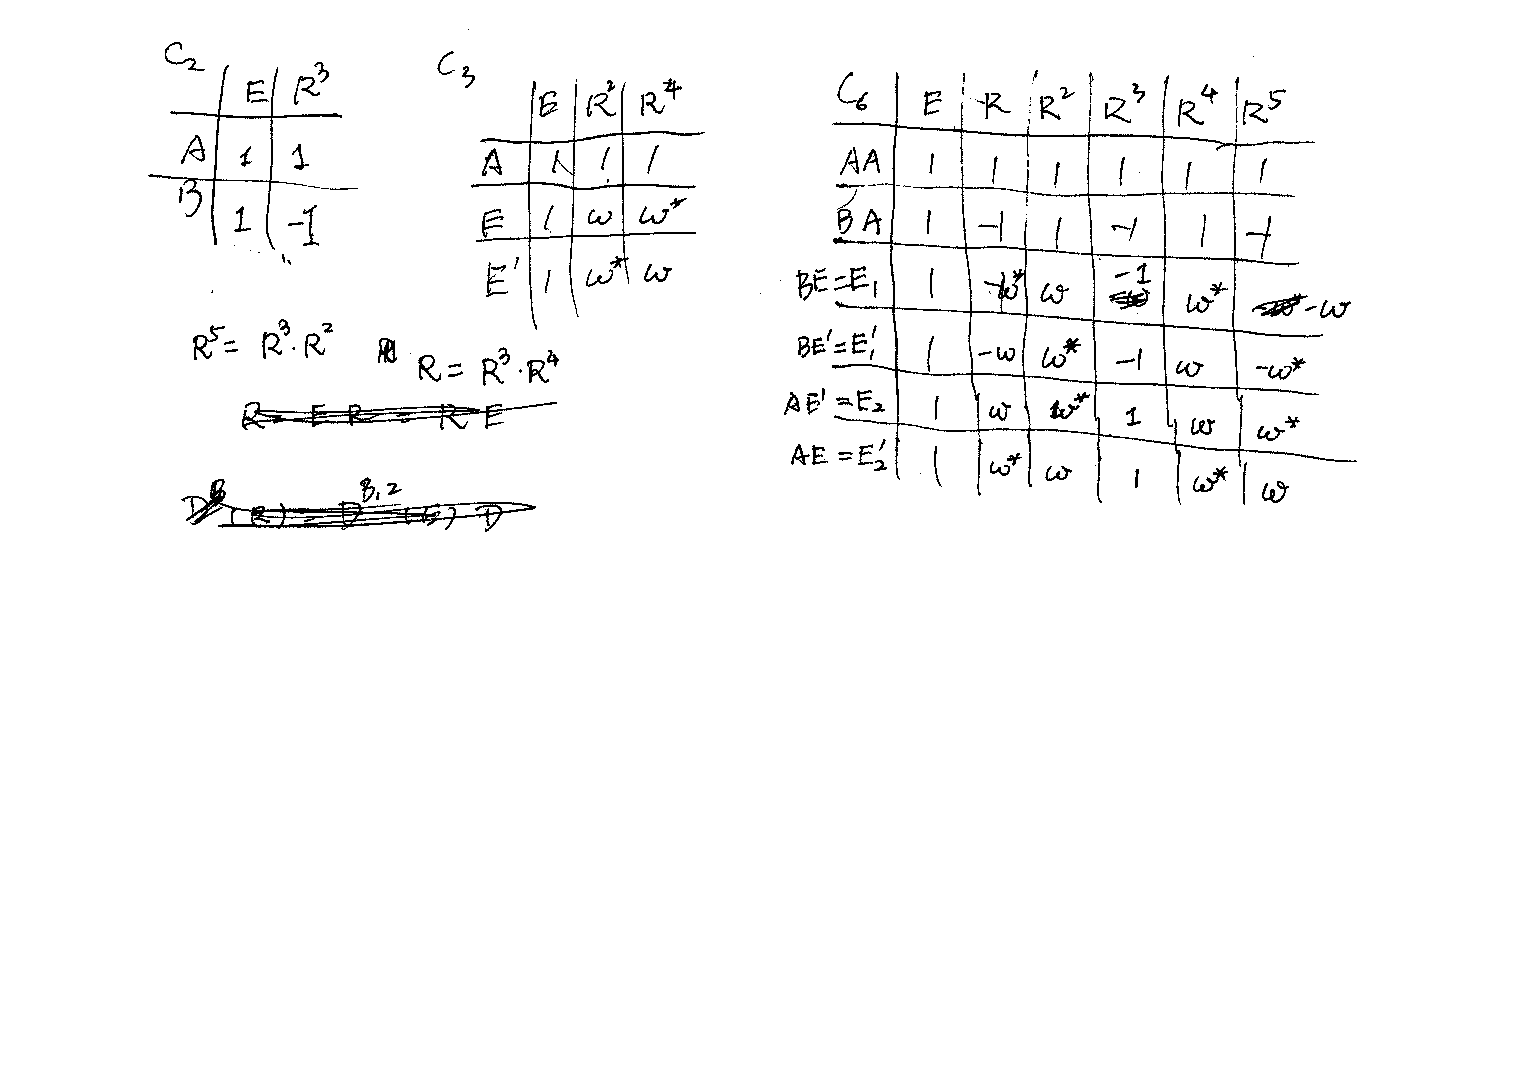
\includegraphics[width=0.8\linewidth]{scans/get-C6-character.pdf}
    \caption{Get $C_6$ Character table}
\end{figure}
\subsection{Dihedral Group \texorpdfstring{$D_n$}{}}
\label{sec:Dihedral-Group}
\begin{defi}[Dihedral Group $D_n$]
\nomenclature{Dihedral Group $D_n$}{\nomrefpage.}
    Dihedral group $D_n$ is the symmetric group of regular $n$-gons
    for $n\geq 3$. For $n=1/2$, it is usually not defined. I found that
    in book \cite{book}, $D_2$ is isomorphic to Klein Group, $D_1$ is
    of course the trivial group.
\end{defi}

But we can have another more mathematical definition of Dihedral
group. To introduce that definition, let me first explain some facts
and discuss a little bit about its conjugacy classes.

There is some important difference between the case when $n$ is odd
and when $n$ is even. When $n$ is odd, the $2$-fold axis are all
linked with the vortices of the $n$-polygon. On the contrary, when $n$
is even, there is two different $2$-fold axis. The first $n/2$
$2$-fold axises are those linked with the vortices, the second $n/2$
$2$-fold axises are those cutting through the opposite edges. 

\subsubsection{Conjugacy Classes}
Note that by fact \ref{fact:20161010-srs} one can see that such
difference mentioned will make the two classes of $2$-fold axises in
even $n$ each form their own conjugacy class. On the contrary, by the
same fact \ref{fact:20161010-srs} one sees that when $n$ is odd, all
the $2$-fold axises are in the same conjugacy class. Note that a
reflection is its own inverse, so in either cases ($n$ odd or even),
we have found self-conjugate classes.

The next conjugacy classes are about rotation. Denotes one $2\pi/n$
rotation around the $N$-fold axis by $T$, then by this very same fact
\ref{fact:20161010-srs}, $T$ and $T^{-1}$ lies in the same conjugacy
class, related by a reflection around a $2$-fold axis. This is obvious
a self-conjugate class. (Note that, when only $2\pi/n$ rotation is
considered, they form an abelian group and each rotation forms a
conjugacy class.) Similarly for the conjugacy class $\{T^m, T^{-m}\}$,
where $m$ is an integer.

In summary, this discussion shows that the conjugacy classes (all are
self-conjugate) in $D_n$
are:
\begin{fact}
    When $n$ is odd (Let $n=2n'+1$): The identity class, the class of
    all $2$-fold axis. The class of $\{ T^m, T^{-m}\}$, where
    $m=1,2,\cdots, n'$. (Why $m\leq n'$? Think about the case when
    $n=5,n'=2$.). In total $n'+2=\frac{n+3}{2}$ conjugacy
    classes/irreducible representations. All conjugacy classes are
    self-conjugate.
\end{fact}
\begin{fact}
    When $n$ is even (Let $n=2n'$): The identity class, the two
    classes of all $2$-fold axis, as discussed above. The class of
    $\{ T^m, T^{-m}\}$, where $m=1,2,\cdots, n'$. In total
    $n'+3=\frac{n+6}{2}$. All conjugacy classes are self-conjugate.
\end{fact}

\subsubsection{Formal definition of \texorpdfstring{$D_n$}{}}

Having discussed about conjugacy classes, one sees that $D_n$ can be
defined by generators.  Clearly, when $n$ is odd, $D_n$ is generated
by one rotation $2\pi/n$ and one reflection (denoted $C'_2$ in the
book \cite{book}). When $n$ is even, one might thinks that we have
three generators, i.e. the rotation by $2\pi/n$, one reflection about
vortex $C'_2$, and one reflection about middle of edges $C''_2$. But
actually it only needs two. The reflection about middle of edges can
be produced by the rotation and the reflection about vortex, or vice
versa. See this note for example:

\begin{figure}[H]
    \centering
    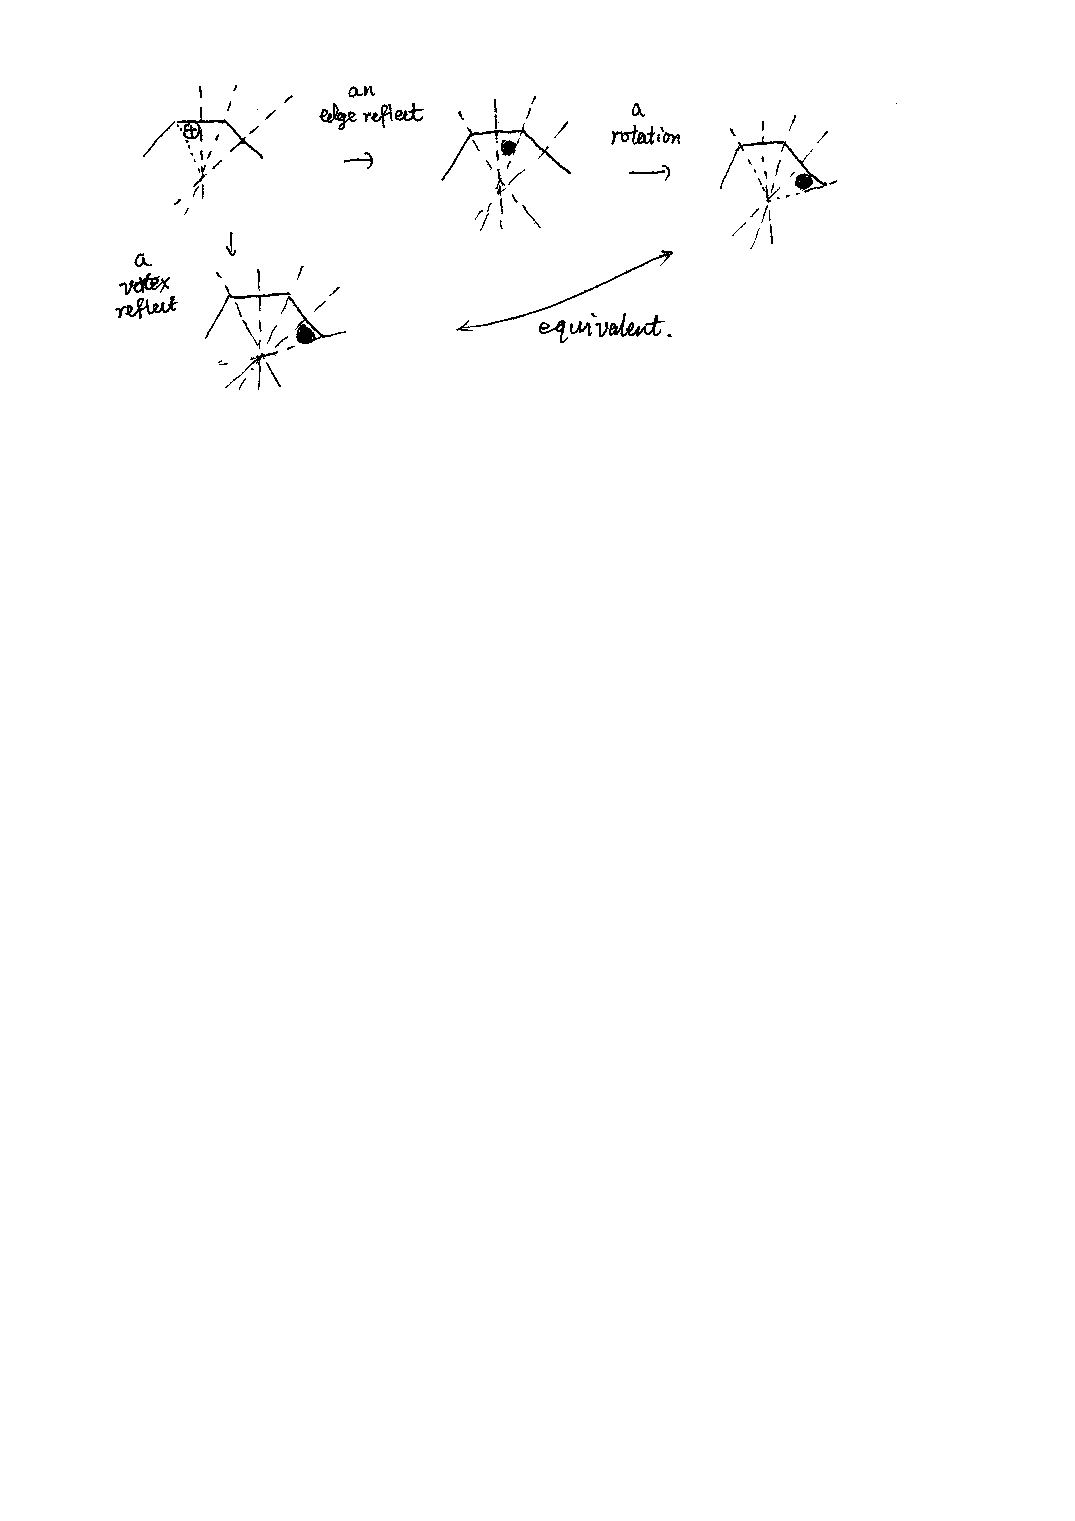
\includegraphics[width=0.8\linewidth]{scans/relate-edge-vortex.pdf}
    \caption{relate-edge-Vortex}
\end{figure}
So all in all, $D_n$ can be generated by just two elements. They are:
\begin{fact}
\label{fact:point-group-formal-def-dn}
\begin{align}
    D_n &\equiv \braket{R,S|R^n=1,S^2=1,SRS^{-1}=R^{-1}} \\
        &\equiv \braket{R,S|R^n=1,S^2=1,(SR)^2=1}
\end{align}
Here the first line symbolizes that rotation $R$ and $R^{-1}$ are in
the same conjugacy class. The second is more beautiful and symbolizes
that a roto-reflection is idempotent.
\end{fact}

Observe that by this definition, it's easy to prove that
\begin{align}
    SR &= R^{-1}S \\
    SR^{-1} &= RS
\end{align}
which are all physically intuitive. A more sophisticated law is
also physically easy to see
\begin{fact}
    \begin{equation}
        S_m R^n = R^{-n}S_m
    \end{equation}
\end{fact}
But I here give a mathematical derivation of the above formula:
\begin{proof}
    Assume $n$ is add.

    Pick a reference point in the $n$-polygon, label its vortex as $0$. Then
    let $S_0= S$ be the reflection about this vortex axis. Then label
    all the remaining vortex $2$-fold axises in the same direction as
    $R$ as $1,2,\cdots,n-1$. Obviously we have:
    \begin{align}
        S_1 &= RS_0 R^{-1} = RSR^{-1} \nonumber\\
        S_2 &= RS_1 R^{-1} = R^2 S R^{-2} \nonumber\\
        \cdots & \nonumber \\
        S_{m} &= R^{m} S R^{m}
    \end{align}
    where $m=1,2,\cdots,n-1$. Then
    \begin{align*}
        S_m R^n &= R^m S R^{-m} R^n \\
          &= R^m S R^n R^{-m}\\
          &= R^m R^{-n} S R^{-m} \\
          &= R^{-n} S_m
    \end{align*}

    When $n$ is odd, the proof is the same, except that now $S_{2m}$ is a
    vortex reflection, and $S_{2m+1}$ is an edge reflection
    ($m=0,1,\cdots (n/2-1)$). Notice that $S_1= RS_0 = RS$, we easily
    see
    \begin{align}
        S_{2m} &= R^m S R^{-m} \\
        S_{2m+1} &= R^{m+1} S R^{-m}
    \end{align}
    and the rest of the proof is the same.
\end{proof}

\subsubsection{Invariant Subgroups} (\textbf{pp.30 of \cite{book}})
By the distinction between edge and vortices type of $2$-fold axises
discussed before, one can see that there is difference in invariant
subgroup when $n$ is odd or even. For example, when $n=5$ is odd,
$D_5$ has only $C_5$ as a notrivial subgroup. But when
$n=6$ is even, it has $C_6$ (then $C_2$ and $C_3$), two copies of
$D_3$ (each formed by edge and vortex type of $2$-fold axis).

More generally, there importnat subgroup of index for $D_n$. When $n$
is odd (let $n'2n'+1$), there are one subgroup of index $2$, i.e.
$C_n'$. When $n$ is even (let $n'=n/2$), there are three invariant
subgroup of index $2$: $C_n'$, $D_n$, and $D_n'$. Denote $n$ $2$-fold
axis as $S_j$, rotation around $n$-fold axis by $2\pi/n$ as $T$,
then:
\begin{align}
    D_n &= \{E, T^2,T^4,\cdots,T^{2n-2},S_0,S_2,\cdots,S_{2n-2}\} \\
    D_n' &= \{E, T^2,T^4,\cdots,T^{2n-2},S_1,S_3,\cdots,S_{2n-1}\}
\end{align}
Note that this list is not complete. For example, $D_6$ contains other
nontrivial invariant subgroups, listed in page 30 of \cite{book}.

\subsubsection{Character Table} (\textbf{pp.66 of \cite{book}})

For $D_2$, it is isomorphic to the group
$\{1,\sigma,\tau,\sigma\tau\}$, where $\sigma$ is spatial inversion,
$\tau$ is time-reversal. Notice that this group is abelian, so it
obvious has $4$ irreducible representations. It is easy to get its
character table, which may be found on page 66, table 3.6 of
\cite{book}.

For $D_3$, it is non-abelian. As discussed previously, it has $3$
conjugacy classes, so it has 3 irreducible representations. Notice
that $D_3/C_3 \cong C_2$, so it inherets the two simple irreducible
representations of $C_2$. This gives two lines in the character
table. Also, $6-1^2-1^2=2^2$, so we have one $2$-dimensional
irreducible representation left.  Next, by fact
\ref{fact:character-of-identity}, we can determine one element in the
character for $2$-dimensional irreducible representation. The rest two
empty blanks can be filled using the orthogonal relations for the
character table.
\begin{figure}[H]
    \centering
    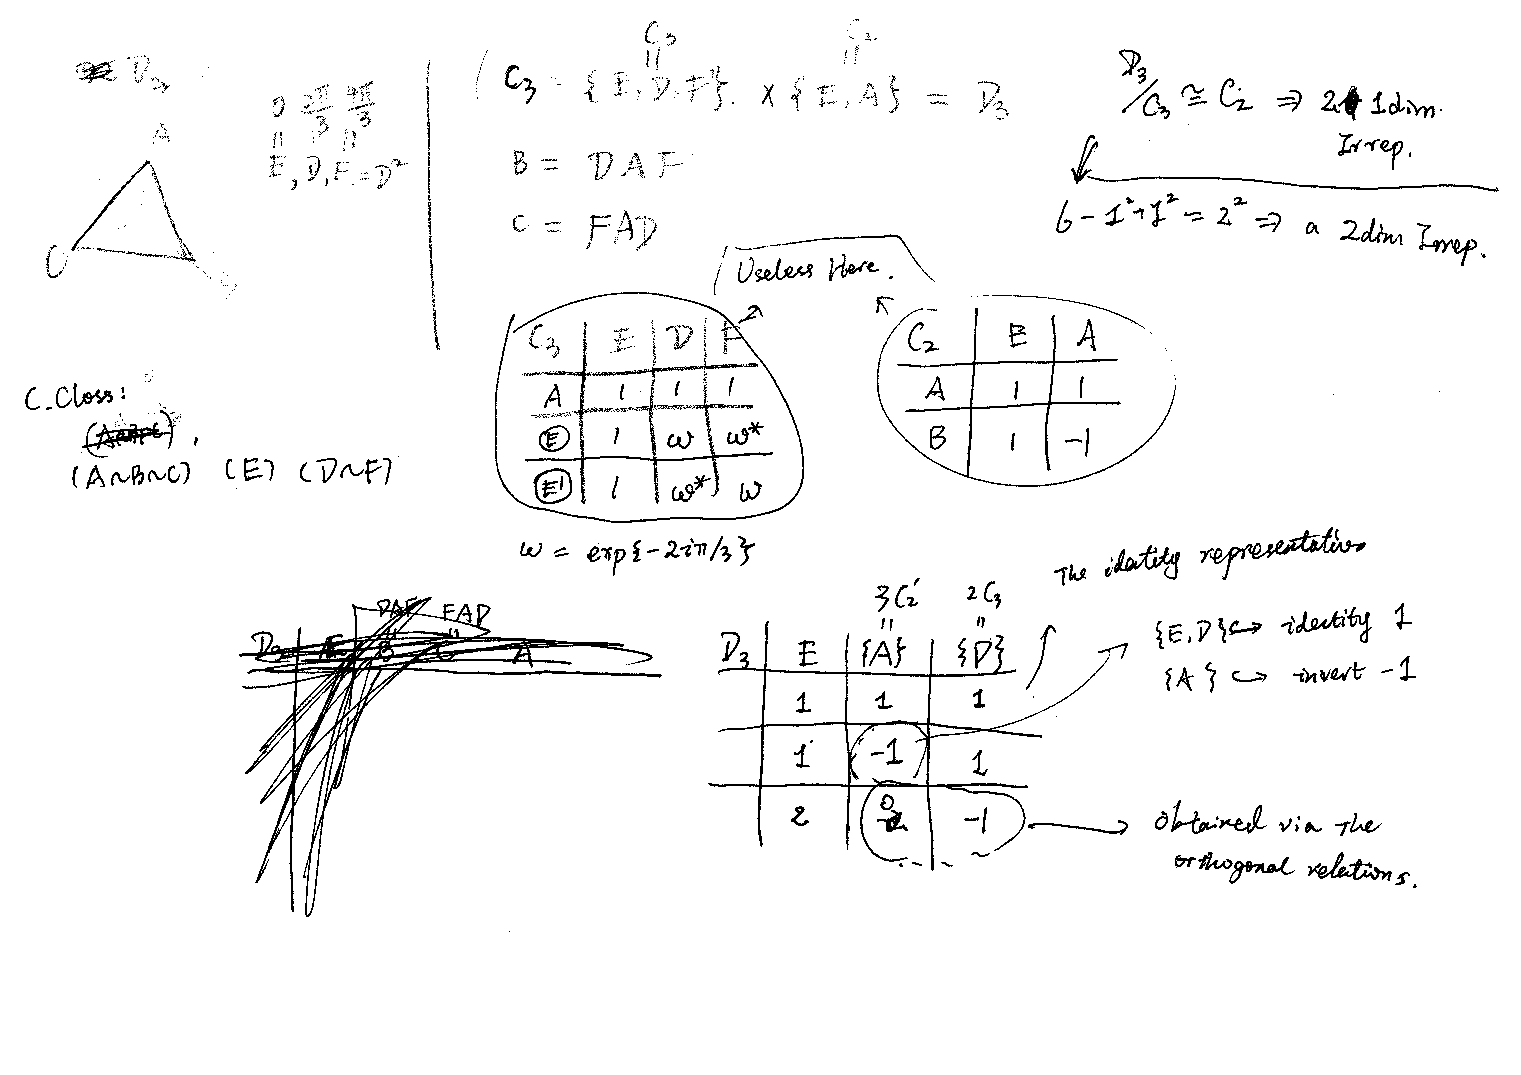
\includegraphics[width=0.8\linewidth]{scans/get-D3-character.pdf}
    \caption{Get $D_3$ Character table}
\end{figure}

For general $D_n$, see the part for irreducible representations.

\subsubsection{Irreducible representation} 

(\textbf{pp.71-74 of \cite{book}}) 

The general procedure is to use the invariant subgroup of index $2$
mentioned above to get the $1$-dimensional representations. And use
the relation $\sum_j m_j^2 = |D_n|$ and $\sum_j 1 = $ number of
conjugacy class to get the dimensional of remaining irreducible
representations. Finally use subgroup $C_n$ to construct those
representations (induced representation) and reduce these into
irreducible ones. But how to reduce them into irreducible one is
actually the most difficult part, in my opinion.

I present only vague discussion below. For details, please to ...
actually I don't know which book. The textbook \cite{book} is too
concise. Perhaps I should find some more detailed books.
% TODO Add better books.

For odd $n$, let $n=2n'+1$. We have:
\begin{align}
    \sum_{j=1}{n'+2} m_j^2 = 4n'+2
\end{align}

There is two $1$-dimensional irreducible representations, formed using
the invariant subgroup $C_{2n'+1}$. Since $4n'+2 = 2^2 n'+2$, one
guesses\footnote{Actually, the remaing ones can satisfy our condition
    only if they are $2$-dimensional. A $1$-dimensional would means an
    additional invarian subgroup of index $2$, which is not true. A
    $3$-dimensional would demand an additional $1$-dimensional
    representation to balance and get a even number. So
$2$-dimensional is the only possibility.}, that the remaining ones are
$n$ $2$-dimensional irreducible representations. They are constructed
(construction process could be found in \cite{book}) to be (notice
$D_{2n'+1}$ is generated by $T_{2n'+1}$, the rotation
$2\pi/(2n'+1)$, and $C'_2$, any one of the $2$-fold reflection):
\begin{align}
    \bar{D}^{E_j}(C_{n}) &=\left( \begin{array}{cc}
    \cos(\frac{2j\pi}{n}) & -\sin(\frac{2j\pi}{n}) \\
    \sin(\frac{2j\pi}{n}) & \cos(\frac{2j\pi}{n}) \\
        \end{array} \right) \\
    \bar{D}^{E_j}(C'_{2}) &= \left( \begin{array}{cc}
                 1 & 0 \\
                 0 & -1 \\ 
                 \end{array} \right)
\end{align}
where $j=1,2,\cdots,n$.

The case for even $n$ is simialr (let $n'=n/2$). Except that now it
has three invariant subgroup of index $2$ (see dicusson about invariant
subgroup above). So it has $2+2+2-2=4$ $1$-dimensional irreducible
representations ($-2$ for the repeated identity representation), and
$n'-1$ $2$-dimensional irreducible representations.
(we have $\sum_{j=1}^{n'+3}m_j^2 = 4n' = (n-1)2^2 + 4\cdot 1$.)
The result is exactly the same as in the the add $n$ case, and this is
why I did not write $2n'+1$ but use $n$ in the above equations.


\subsection{T-group}

\nomen{$T$ group} is the group of the symmetry of tetrahedrons. It is
a subgroup of $O$, the symmetry of cubic or octahedron (will % TODO ).

A graph is provided in the page 33 of \cite{book}.  Part of this work
has been done in the mid-term exam and is not repreated here.

The conjugacy classes:
$\{E\}$ and $\{3C_2\}$, $\{4C'_2\}$, $\{4C'^2_2\}$.

\paragraph{Character Table}
It has a subgroup of $D_2$, which can be seen from analysing the
number of elments in conjugacy classes. $D_2$ is just $C_3$ discussed
before, and it has three 1D representations. So first three line of
the character is simple to get.

The remaing representation is $3$-dimensional, so we can again fill
one element of the character table. The rest can be easily filled by
the orthogonal relations.

Details on page 66 and 33 of \cite{book}.


\section{20161121}

Now we consider the classification of wavefunctions using the
symmetric groups we have known. In general, we need a symmetry, its
symmetry group, and the (irreducible) representation matrices.
During the classification, the representation space is the space
spanned by the set of degenerate wave functions $\psi_\rho$
($\rho=1,\cdots,m$), $\mathcal{L}_E=\operatorname{span}\{\psi_\rho\}$.

assuming we have
\begin{equation}
    H\psi_\rho(x) = E\psi_\rho(x)
\end{equation}

The $\psi_\rho$ satisfies orthogonal relations.
Now we do a spatial transformation, and assume this transformation
satisfy the symmetry of the Hamiltonian ($HP_R = P_R H$). Thn we have:
\begin{equation}
    P_R(\psi_\rho(x)) = \psi_\rho(R^{-1} x) = \sum_\lambda \psi_\lambda
    D_{\lambda\rho}(x)
\end{equation}
In this way, we obtain a representations of our symmetry. Usually,
$P_R$ is unitary, and since our basis $\psi_\rho$ is orthonormal, the
matrix $D$ is unitary. Now we want to find those irreducible
representations, so we do:
\begin{align}
    X^{-1} D(R) X = \oplus_j a_j D^j(R)
\end{align}
where $R\in G$, $D^j$ labels those irreducible representations, $X$ is
some matrix that we do not know now.

$a_j$ can be calculated using previous orthogonal relationships. More
specifically, we have
\begin{equation}
    a_j = \frac{1}{|G|} \sum_{R\in G} (\chi^j(R))^* \chi(R)
\end{equation}

Now we are interested in geting $X$. Notice that
\begin{align*}
    X^{-1} D(R) X = \oplus_j a_j D^j(R)
\end{align*}
tells us something about $X$. Let $X=X_{a,b}$. Here $1\leq a \leq m$.
$b$ can be labeled by $j,\mu,\gamma$, i.e. the irreducible
representation it is inside ($j$), did this irreducible representation
repeats more than one time ($\gamma$), which element is it ($\mu$). So
we have the new basis $\Psi$ related to the odd basis $\psi$ as
\begin{align}
    P_R(\Psi^j_{\mu\gamma}(x)) &= \sum_\nu
    \Psi^j_{\nu\gamma}(x)D^j_{\nu\mu}(R) \\
    \Psi^j_{\mu\gamma} &= \sum_{\rho} \psi_\rho X_{\rho,j\mu\gamma} \\
    \psi_\rho &= \sum_{j\mu\gamma} \psi^{j}_{\mu\gamma}
    (X^{-1})_{j\mu\gamma,\rho}
\end{align}

we have the theorem
\begin{thm}[W-E]
    \begin{itemize}
        \item Those belong to different irreducible representations
            are orthogonal
        \item Those belong to the same irreducible representation, but
            in different row are orthogonal
        \item Those belong to the same irreducible representation, the
            same row, has inner product independent of the index
    \end{itemize}
\end{thm}

Let $\psi^j_\mu$ and $\phi^k_\rho$ belong to $D^j_\mu$ and $D^k_\rho$.
Then 
$P_R \psi^j_\mu= \sum_\nu \psi^j_\nu D^j_{\nu\mu}(R)$,
$P_R \phi^k_\rho= \sum_\lambda \psi^k_\lambda D^j_{\lambda\nu}(R)$

Define $X^{jk}_{\rho\mu} := \braket{\phi^k_\rho|\psi^j_\mu}$.

\begin{align}
    \braket{\phi^k_\rho|P_R\psi^j_\mu} = \sum_\nu
    \braket{\phi^k_\rho|\psi^j_\nu} D^j_{\nu\mu}(R) = (X^{jk}
    D^j(R))_{\rho\mu} \\
    \braket{P^{-1}\phi^k_\rho|\psi^j_\mu} = \braket{
    \sum_\lambda\phi^k_\lambda D^k_{\lambda\rho}(R^{-})|\psi^j_\nu}
    \\
    = \sum_\lambda [D^k_{\lambda\rho}(R^{-1})]^*
    \braket{\phi^k_\lambda|\psi^j_\mu} 
    = \sum_\lambda D^k_{\rho\lambda}
    \braket{\phi^k_\lambda|\psi^j_\mu}
    = \sum_\lambda X^{kj}_{j\mu} = (D^k(R)X^{kj})_{\rho\mu}
\end{align}

Comparing two sides, we have
\begin{equation}
    D^k(R) X^{kj} = X^{kj}D^j(R)
\end{equation}
So by Schur lemma, we have when $k\neq j$
\begin{equation}
    X^{kj} = 0
\end{equation}
when $k=j$
\begin{equation}
    X^{jk} = \lambda\id
\end{equation}
the constant $\lambda$ is denoted as $\bra{k}\ket{j}$
so
\begin{equation}
    X^{jk} = \bra{k} \ket{j} \id
\end{equation}
In all
\begin{equation}
    \braket{\phi^k_\rho|\psi^j_\mu} = \delta_{jk} \delta_{\rho\mu}
    \bra{k} \ket{j}
\end{equation}

\subsection{Canonical Degeneracy}
\label{sec:Canonical-Degeneracy}
\begin{defi}[Canonical/Accidential Degeneracy]
\nomenclature{Canonical/Accidential Degeneracy}{\nomrefpage.}
    Assume $H$ has $M$-fold degeneracy, wit corresponding
    representations $D(G)$. If the representation is irreducible, then
    the degeneracy is called canonical, otherwise it is called
    accidential.
\end{defi}

Assume we have $[P_R,H_0]=0$, $[P_R,H_1]=0$. 
\begin{align}
    P_R \psi^j_\mu = \sum_\nu \psi^j_\nu D^j_{\nu\mu}(R)\\
    H_0 \psi^j_\mu = E^j \psi^j_\mu \\
    P_R H_1 \psi^j_\mu = H_1 P_R \psi^j_\mu = H_1 \sum_\nu \psi^j_\nu
    D^j_{\nu\mu}(R) = \sum_\nu (H_1\psi^j_\nu) D^j_{\nu\mu}(R) \\
\end{align}
By theorem
\begin{align}
    \braket{\psi^j_\nu|H_1 \psi^j_\nu} = \bra{j}\ket{j}\id = \Delta
    E^j \delta_{\nu\mu}
\end{align}
So the first order correction does not remove the degeneracy. For the
higher order correction, the case will be the same. Here only an
argument is given. We consider the process $H_0 + \lambda H_1$, from
$\lambda=0$ to $\lambda=1$, in this process, if $\lambda$ varies
adiabatically, then the degenerate function will keep their degeneracy
in the gradually process if the Hamiltonian is good enough. 

For \textbf{accidental degeneracy}, for $j\neq i$
\begin{align}
    \braket{\psi^i_\nu|H_1 \psi^i_\mu} = \delta_{\nu\mu} \Delta E^i \\
    \braket{\psi^j_\nu|H_1 \psi^j_\mu} = \delta_{\nu\mu} \Delta E^j \\
\end{align}
In general, $\Delta E^i$ and $\Delta E^j$ is not the same. If they are
the same, then there may be additional symmetry that we have not yet
discovered.

For $j=i$, 
\begin{equation}
P_R \psi^j_{\nu a} = \sum_\nu \psi^j_{\nu a} D^j_{\nu\mu}(R)
\end{equation}
\begin{align}
    \braket{\psi^j_{\mu a} | H_1 |\psi^j_{\nu b}}  = 
\end{align}

Example

\section{20161128}
\label{sec:20161128}
After some work, I realize that it is impractical to follow the
teacher's class with notes. Therefore I will write here just some
important formulae, as a preparation for exams.

Pauli matrices
\begin{align}
    &\sigma_1 =\begin{pmatrix}
        0 & 1\\ 1 & 0
    \end{pmatrix}\\
    &\sigma_2 = \begin{pmatrix}
        0& -i \\ i & 0
    \end{pmatrix} \\
    &\sigma_3 = \begin{pmatrix}
    1 & 0 \\ 0 & -1
    \end{pmatrix}\\
    &\sigma_a \sigma_b = \delta_{ab} \id + i\sum_c
    \varepsilon_{abc}\sigma_c \\
    &\Tr{\sigma_a} =0 \\
    &\Tr{\sigma_a \sigma_b} =2\delta_{ab} \\
    &\exp{-i\omega \sigma_2} =\id \cos{\omega}-i\sigma_2\sin{\omega}
    = \begin{pmatrix}
        \cos{\omega} & -\sin{\omega} \\
        \sin{\omega} & \cos{\omega}
    \end{pmatrix} \\
    &R(\vec{e_3},\omega)= \exp{-i\omega T_3}= \begin{pmatrix}
        \cos{\omega} & -\sin{\omega} & 0 \\
        \sin{\omega} & \cos{\omega} & 0 \\
        0 & 0 & 1
    \end{pmatrix},\quad T_3 = \begin{pmatrix}
        0 & -i & 0 \\
        i & 0 & 0 \\
        0 & 0 & 0
    \end{pmatrix} \\
    & R(\vec{e}_1,\omega) = \exp{-i\omega T_1} = \begin{pmatrix}
        1 & 0 & 0 \\
        0 & \cos{\omega} & -\sin{\omega} \\
        0 & \sin{\omega} & \cos{\omega} 
    \end{pmatrix},\, T_1 = \begin{pmatrix}
        0 & 0 & 0 \\
        0 & 0 & -i \\
        0 & i & 0
    \end{pmatrix}\\
    & R(\vec{e}_2,\omega) = \exp{-i\omega T_2} = \begin{pmatrix}
        \cos{\omega} & 0 & \sin{\omega} \\
        0 & 1 & 0 \\
    -\sin{\omega} & 0 & \cos{\omega} 
    \end{pmatrix},\, T_2 = \begin{pmatrix}
        0 & 0 & i \\
        0 & 0 & 0 \\
        -i & 0 & 0
    \end{pmatrix}\\
    & (T_a)_{bc}= -i\varepsilon_{abc} \\
    & S(\phi,\theta) = \begin{pmatrix}
    \cos{\phi}\cos{\theta} & -\sin{\phi} & \cos{\phi}\sin{\theta} \\
    \sin{\phi}\cos{\theta} & \cos{\phi} & \sin{\phi}\sin{\theta} \\
    -\sin{\theta} & 0 & \cos{\theta}
    \end{pmatrix} \\
    & S(\phi,\theta) \begin{pmatrix}
        0 \\ 0 \\ 1
    \end{pmatrix} = \begin{pmatrix}
        \cos{\phi}\sin{\theta} \\ \sin{\phi}\sin{\theta} \\ \cos{\theta}
    \end{pmatrix} = \begin{pmatrix}
        n_1 \\ n_2 \\ n_3
    \end{pmatrix}\\
    & R(\vec{n},\omega) =
        S(\phi,\theta)R(\vec{e_3},\omega)S(\phi,\theta)^{-1}
        =\exp{-i\omega\vec{n}\vdot\vec{T}}
        = \exp{-i\sum_a \omega_a T_a} \\
    & R(\vec{n},\omega) = R(-\vec{n},2\pi-\omega) \\
    & S T_3 S^{-1} = \vec{n}\vdot\vec{T}
\end{align}
\begin{fact}
    The character $\chi$ of $SO(3)$ is a function of $\omega$ only. In
    fact:
    \begin{equation}
        \chi(R(\vec{n},\omega)) = 1+2\cos{\omega}
    \end{equation}
\end{fact}
\begin{enumerate}
    \item $R\in G$, $\# G=g$

        $ R(1):=R(r_1,r_2,\cdot,r_g)$
    \item $R(r)S(s)=T(t)$,

        $f(r,s)=t$, $f:(Space)\otimes(Space)\to (Space)$.

        

        $t_j = f_j(r_1,\cdot,r_g,s_1,\cdot,s_g)=f_j(r,s)$
\end{enumerate}

\begin{align}
    & P_R\psi(x)=\psi(R^{-1}x) \\
    & I^{(0)}_j = -i\sum_a 
        \eval{\frac{\partial (Ax)_a}{\partial \alpha_j}}_{\alpha=0}
        \frac{\partial }{\partial x_a} \\
    & P_A\psi(x) = \psi(x)-i\sum_{j=1}^g \alpha_j I^{(0)}_j\psi(x)
\end{align}
\section{Anchor}
\label{sec:Anchor}
\begin{thebibliography}{1}
    \bibitem{book} Zhongqi Ma, Group Theory in Physics
    \bibitem{math.se_1_lenz_vector} \href{physics.stackexchange.com/questions/18088/what-symmetry-causes-the-runge-lenz-vector-to-be-conserved}{What symmetry causes the Runge-Lenz vector to be conserved?}
    \bibitem{Ludeling} Lecture Notes for physics751: Group Theory (for
    Physicists), by C Ludeling.
    \href{http://www.th.physik.uni-bonn.de/nilles/people/luedeling/grouptheory/data/grouptheorynotes.pdf}{Link}
    \bibitem{lang-algebra} Serge Lang. Algebra. Revised 3rd. Springer.
\end{thebibliography}
\printnomenclature
\section{License}
The entire content of this work (including the source code
for TeX files and the generated PDF documents) by 
Hongxiang Chen (nicknamed we.taper, or just Taper) is
licensed under a 
\href{http://creativecommons.org/licenses/by-nc-sa/4.0/}{Creative 
Commons Attribution-NonCommercial-ShareAlike 4.0 International 
License}. Permissions beyond the scope of this 
license may be available at \url{mailto:we.taper[at]gmail[dot]com}.
\end{document}
